%% GENERATED by tools/from_docs.py from stepss-docs. Do not edit by hand:
%% edit the page named below in stepss-docs and regenerate.
%% source: stepss-docs/src/content/docs/models/custom-injectors.md

\chapter{Injector models}\label{doc:model-inj}

RAMSES custom injector models represent loads, induction machines, inverter-based resources (IBR), and battery energy storage systems (BESS) connected to network buses.

\begin{docsnote}{Usage in Dynamic Data Files}

Injector models are defined with the \texttt{INJEC} keyword as standalone records in the dynamic data file. The syntax is:

\begin{Verbatim}
INJEC model_name inj_name bus FP FQ P Q param1 param2 ... ;
\end{Verbatim}

Where \texttt{model\_name} is the model identifier, \texttt{inj\_name} is a unique instance name, \texttt{bus} is the connection bus, \texttt{FP}/\texttt{FQ} are participation factors, and \texttt{P}/\texttt{Q} are initial values in MW/Mvar (one of each pair must be zero, either the fraction or the absolute power).

Recognised injector model names (case-sensitive):

\begin{itemize}
\tightlist
\item
  \textbf{Uppercase short names} (no prefix): \texttt{LOAD}, \texttt{RESTLD}, \texttt{THEVEQ}, \texttt{INDMACH1}, \texttt{INDMACH2}, \texttt{SVC\_GENERIC1}.
\item
  \textbf{Prefixed names}: RAMSES adds the \texttt{inj\_} prefix automatically: \texttt{VFAULT}/\texttt{inj\_VFAULT}, \texttt{vfd\_load}/\texttt{inj\_vfd\_load}, \texttt{PQ}/\texttt{inj\_PQ}, \texttt{IBG}/\texttt{inj\_IBG}, \texttt{WT3}/\texttt{inj\_WT3}, \texttt{WT4}/\texttt{inj\_WT4}, \texttt{BESS}/\texttt{inj\_BESS}, \texttt{GFOL}/\texttt{inj\_GFOL}, \texttt{GFOR}/\texttt{inj\_GFOR}, \texttt{PMU}/\texttt{inj\_PMU}.
\end{itemize}

All of the above are built into every RAMSES distribution (standalone executable and shared library used by stepss). \texttt{INDM1} and \texttt{PV}, documented below, have been callable since 3.79; before that they were compiled under no name. \texttt{inj\_norton} is excluded from the build entirely and is not available: it calls a Python bridge (\texttt{initialize\_model\_instance}, \texttt{call\_python\_evaluate}) that is not part of this source tree.

\textbf{Note on case sensitivity.} Match the case used above exactly. The uppercase short names must be uppercase. For the prefixed family, \texttt{vfd\_load} and \texttt{VFAULT} use those exact cases. Most others follow the convention \texttt{inj\_\textless{}UPPERCASE\textgreater{}} (e.g.~\texttt{inj\_PQ}, \texttt{inj\_GFOR}).

\end{docsnote}

\begin{center}\rule{0.5\linewidth}{0.5pt}\end{center}

\section{Load Models}\label{model-inj:load-models}

\subsection{\texorpdfstring{LOAD (\texttt{inj\_load}): Exponential Recovery Load}{LOAD (inj\_load): Exponential Recovery Load}}\label{model-inj:load-inj_load-exponential-recovery-load}

\subsubsection{Description}\label{model-inj:description}

The exponential recovery load model captures the transient and steady-state voltage and frequency dependency of aggregated loads. Immediately after a voltage disturbance, the load behaves according to a transient voltage exponent; it then recovers exponentially to a steady-state behaviour described by a different exponent. The model supports separate active (\(P\)) and reactive (\(Q\)) power recovery dynamics, each with individual minimum/maximum limiters on the recovery variable.

\begin{figure}[htbp]
\centering
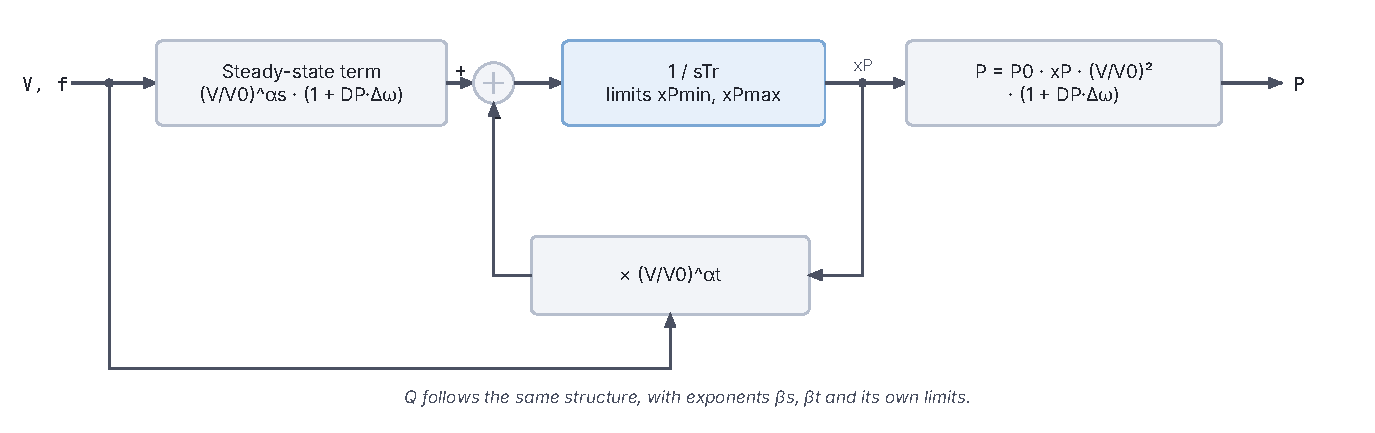
\includegraphics[width=0.98\linewidth]{figures/inj-load-light}
\caption{Exponential recovery load block diagram.}
\end{figure}

\subsubsection{Scientific Description}\label{model-inj:scientific-description}

The model is parameterized in terms of initial active and reactive conductance/susceptance, \(G_0 = P_0/V_0^2\) and \(B_0 = -Q_0/V_0^2\). Two recovery state variables \(x_P\) and \(x_Q\) evolve according to:

\[\dot{x}_P = \frac{1}{T_r}\left[\left(\frac{V}{V_0}\right)^{\alpha_s} \left(1 + D_P\,\Delta\omega\right) - x_P \left(\frac{V}{V_0}\right)^{\alpha_t}\right]\]

\[\dot{x}_Q = \frac{1}{T_r}\left[\left(\frac{V}{V_0}\right)^{\beta_s} \left(1 + D_Q\,\Delta\omega\right) - x_Q \left(\frac{V}{V_0}\right)^{\beta_t}\right]\]

where \(\Delta\omega = \omega_{\mathrm{COI}} - 1\) is the per-unit speed deviation, \(V\) is the bus voltage magnitude, \(V_0\) is the initial voltage, \(\alpha_t, \beta_t\) are transient exponents, \(\alpha_s, \beta_s\) are steady-state exponents, and \(T_r\) is the load recovery time constant. The injected currents are then:

\[i_x = G_0\, x_P\, v_x\left(1 + D_P\,\Delta\omega\right) - B_0\, x_Q\, v_y\left(1 + D_Q\,\Delta\omega\right)\]

\[i_y = G_0\, x_P\, v_y\left(1 + D_P\,\Delta\omega\right) + B_0\, x_Q\, v_x\left(1 + D_Q\,\Delta\omega\right)\]

When the recovery variable hits its limit (due to e.g.~Stalling or complete voltage collapse), the limit is held until the direction of the derivative reverses.

\subsubsection{Parameters}\label{model-inj:parameters}

\begin{small}\begin{longtable}[]{@{}
  >{\raggedright\arraybackslash}p{(\linewidth - 8\tabcolsep) * \real{0.1047}}
  >{\raggedright\arraybackslash}p{(\linewidth - 8\tabcolsep) * \real{0.1832}}
  >{\raggedright\arraybackslash}p{(\linewidth - 8\tabcolsep) * \real{0.5961}}
  >{\raggedright\arraybackslash}p{(\linewidth - 8\tabcolsep) * \real{0.1160}}
@{}}
\toprule\noalign{}
\begin{minipage}[b]{\linewidth}\raggedright
\#
\end{minipage} & \begin{minipage}[b]{\linewidth}\raggedright
Name
\end{minipage} & \begin{minipage}[b]{\linewidth}\raggedright
Description
\end{minipage} & \begin{minipage}[b]{\linewidth}\raggedright
Unit
\end{minipage} \\
\midrule\noalign{}
\endhead
\bottomrule\noalign{}
\endlastfoot
1 & \texttt{DP} & Frequency sensitivity of active power & pu/pu \\
2 & \texttt{A1} & Proportion of type-1 component in \(P\) & \\
3 & \texttt{alpha1} & Transient voltage exponent for \(P\) (type 1) & \\
4 & \texttt{A2} & Proportion of type-2 component in \(P\) & \\
5 & \texttt{alpha2} & Transient voltage exponent for \(P\) (type 2) & \\
6 & \texttt{alpha3} & Transient voltage exponent for \(P\) (type 3, proportion \(= 1-A_1-A_2\)) & \\
7 & \texttt{DQ} & Frequency sensitivity of reactive power & pu/pu \\
8 & \texttt{B1} & Proportion of type-1 component in \(Q\) & \\
9 & \texttt{beta1} & Transient voltage exponent for \(Q\) (type 1) & \\
10 & \texttt{B2} & Proportion of type-2 component in \(Q\) & \\
11 & \texttt{beta2} & Transient voltage exponent for \(Q\) (type 2) & \\
12 & \texttt{beta3} & Transient voltage exponent for \(Q\) (type 3) & \\
\end{longtable}\end{small}

Internal computed parameters include the steady-state exponents for each component (derived from the transient exponents), initial conductance \(G_0\), susceptance \(B_0\), and initial voltage \(V_0\).

\subsubsection{State Variables}\label{model-inj:state-variables}

\begin{small}\begin{longtable}[]{@{}ll@{}}
\toprule\noalign{}
Variable & Description \\
\midrule\noalign{}
\endhead
\bottomrule\noalign{}
\endlastfoot
\texttt{iy} & \(y\)-component of injected current (pu on system base) \\
\texttt{ix} & \(x\)-component of injected current (pu on system base) \\
\texttt{xp} & Active power recovery variable (dimensionless) \\
\texttt{xq} & Reactive power recovery variable (dimensionless) \\
\end{longtable}\end{small}

\textbf{Observables:} \texttt{P}, \texttt{Q}, \texttt{xp}, \texttt{xq}

\subsubsection{Usage Example}\label{model-inj:usage-example}

\begin{Verbatim}
INJEC  LOAD  LOAD1  BUS1  1.  1.  0.  0.  1.5  0.3  1.0  0.2  2.0  0.5  1.8  0.4  2.5  0.1  3.0  2.0  ;
\end{Verbatim}

\emph{Parameters: \texttt{DP\ A1\ alpha1\ A2\ alpha2\ alpha3\ DQ\ B1\ beta1\ B2\ beta2\ beta3}}

\begin{center}\rule{0.5\linewidth}{0.5pt}\end{center}

\subsection{\texorpdfstring{vfd\_load (\texttt{inj\_vfd\_load}): Variable Frequency Drive Load}{vfd\_load (inj\_vfd\_load): Variable Frequency Drive Load}}\label{model-inj:vfd_load-inj_vfd_load-variable-frequency-drive-load}

\subsubsection{Description}\label{model-inj:description-1}

The VFD load model represents aggregate industrial loads driven by variable-frequency drives, where the power consumption exhibits a composite voltage-dependent characteristic with multiple exponential components and frequency sensitivity. It also includes low-voltage protection: below a configurable threshold \(V_{\min}\), the load switches to a constant-admittance representation, preventing numerical difficulties during deep voltage sags.

\subsubsection{Scientific Description}\label{model-inj:scientific-description-1}

The active and reactive powers depend on bus voltage \(V\) and frequency deviation \(\Delta f = f/f_0 - 1\):

\[P = \left(1 + D_P\,\Delta f\right) P_0 \cdot \frac{a_1 V^{\alpha_1} + a_2 V^{\alpha_2} + (1-a_1-a_2)\, V^{\alpha_3}}{a_1 V_0^{\alpha_1} + a_2 V_0^{\alpha_2} + (1-a_1-a_2)\, V_0^{\alpha_3}}\]

\[Q = \left(1 + D_Q\,\Delta f\right) Q_0 \cdot \frac{b_1 V^{\beta_1} + b_2 V^{\beta_2} + (1-b_1-b_2)\, V^{\beta_3}}{b_1 V_0^{\beta_1} + b_2 V_0^{\beta_2} + (1-b_1-b_2)\, V_0^{\beta_3}}\]

Below \(V_{\min}\), an equivalent constant admittance is used:

\[P_{\mathrm{low}} = G_{\mathrm{eq}}\, V^2, \qquad Q_{\mathrm{low}} = -B_{\mathrm{eq}}\, V^2\]

where \(G_{\mathrm{eq}}\) and \(B_{\mathrm{eq}}\) are computed at initialization to ensure continuity at \(V = V_{\min}\). The switch between the two regimes is governed by a piecewise-linear function of \(V\):

\[u = \begin{cases} 0 & V < V_{\min} \\ 1 & V \geq V_{\min} \end{cases}\]

A small voltage filter (time constant 0.003 s) smooths the transition. The frequency deviation can optionally be computed from the local bus frequency (measured via an \texttt{f\_inj} block with time constant \(T_{\mathrm{mes}}\)) or from the system centre-of-inertia speed.

The initial voltage \(V_0\) can differ from the transmission bus voltage if a distribution transformer ratio is implied (set \(V_{\mathrm{init}} \ne 0\) to specify the distribution-side voltage; otherwise the transmission voltage is used directly).

\subsubsection{Parameters}\label{model-inj:parameters-1}

\begin{small}\begin{longtable}[]{@{}
  >{\raggedright\arraybackslash}p{(\linewidth - 8\tabcolsep) * \real{0.1092}}
  >{\raggedright\arraybackslash}p{(\linewidth - 8\tabcolsep) * \real{0.1851}}
  >{\raggedright\arraybackslash}p{(\linewidth - 8\tabcolsep) * \real{0.5926}}
  >{\raggedright\arraybackslash}p{(\linewidth - 8\tabcolsep) * \real{0.1130}}
@{}}
\toprule\noalign{}
\begin{minipage}[b]{\linewidth}\raggedright
\#
\end{minipage} & \begin{minipage}[b]{\linewidth}\raggedright
Name
\end{minipage} & \begin{minipage}[b]{\linewidth}\raggedright
Description
\end{minipage} & \begin{minipage}[b]{\linewidth}\raggedright
Unit
\end{minipage} \\
\midrule\noalign{}
\endhead
\bottomrule\noalign{}
\endlastfoot
1 & \texttt{Dp} & Frequency sensitivity of active power & pu/pu \\
2 & \texttt{a1} & Fraction of type-1 component in \(P\) & \\
3 & \texttt{alpha1} & Voltage exponent of type-1 \(P\) component & \\
4 & \texttt{a2} & Fraction of type-2 component in \(P\) & \\
5 & \texttt{alpha2} & Voltage exponent of type-2 \(P\) component & \\
6 & \texttt{alpha3} & Voltage exponent of type-3 \(P\) component (fraction \(= 1-a_1-a_2\)) & \\
7 & \texttt{Dq} & Frequency sensitivity of reactive power & pu/pu \\
8 & \texttt{b1} & Fraction of type-1 component in \(Q\) & \\
9 & \texttt{beta1} & Voltage exponent of type-1 \(Q\) component & \\
10 & \texttt{b2} & Fraction of type-2 component in \(Q\) & \\
11 & \texttt{beta2} & Voltage exponent of type-2 \(Q\) component & \\
12 & \texttt{beta3} & Voltage exponent of type-3 \(Q\) component & \\
13 & \texttt{Vinit} & Initial distribution-bus voltage (0 = use transmission voltage) & pu \\
14 & \texttt{Vlow} & Voltage threshold for constant-admittance regime (recommended 0.5--0.7) & pu \\
15 & \texttt{foption} & 1 = use local bus frequency; 0 = use COI speed & flag \\
16 & \texttt{Tmes} & Frequency measurement time constant & s \\
\end{longtable}\end{small}

\subsubsection{State Variables}\label{model-inj:state-variables-1}

\begin{small}\begin{longtable}[]{@{}ll@{}}
\toprule\noalign{}
Variable & Description \\
\midrule\noalign{}
\endhead
\bottomrule\noalign{}
\endlastfoot
\texttt{Vreal} & Voltage at equivalent distribution bus \\
\texttt{V} & Filtered distribution-bus voltage (3 ms filter) \\
\texttt{P} & Active power consumed \\
\texttt{Q} & Reactive power consumed \\
\texttt{fbus} & Local bus frequency (used if \texttt{foption=1}) \\
\texttt{df} & Frequency deviation \(\Delta f\) \\
\texttt{u} & Regime switch (1 = above \(V_{\min}\), 0 = constant admittance) \\
\end{longtable}\end{small}

\textbf{Observables:} \texttt{P}, \texttt{Q}, \texttt{df}, \texttt{u}

\subsubsection{Usage Example}\label{model-inj:usage-example-1}

\begin{Verbatim}
INJEC  vfd_load  VFD1  BUS_IND  1.  1.  0.  0.  1.5  0.7  2.0  0.2  1.0  0.5
                                 1.2  0.5  2.5  0.1  1.5  0.8
                                 0.0  0.6  0  0.1  ;
\end{Verbatim}

\begin{center}\rule{0.5\linewidth}{0.5pt}\end{center}

\subsection{\texorpdfstring{RESTLD (\texttt{inj\_restld}): Restorative Load}{RESTLD (inj\_restld): Restorative Load}}\label{model-inj:restld-inj_restld-restorative-load}

\subsubsection{Description}\label{model-inj:description-2}

The restorative load model represents loads that self-restore toward a nominal characteristic after a voltage disturbance. The load's active and reactive powers are governed by two internal recovery variables that evolve dynamically, allowing the simulation to capture the slow restoration of thermostatically controlled loads (heating, cooling) and similar self-restoring demand.

\subsubsection{Scientific Description}\label{model-inj:scientific-description-2}

The recovery variable \(x_P\) for active power satisfies:

\[\dot{x}_P = \frac{1}{T_r}\left[V^{\alpha_s}\left(1 + D_P\,\Delta\omega\right) - x_P\, V^{\alpha_t}\right]\]

with analogous equation for \(x_Q\). Here \(\alpha_s\) and \(\alpha_t\) are the steady-state and transient voltage exponents respectively. Limiters \([x_{P,\min},\, x_{P,\max}]\) are applied. The injected currents are expressed as:

\[i_y = -B_0\left(1 + D_Q\,\Delta\omega\right) x_Q\, v_x + G_0\left(1 + D_P\,\Delta\omega\right) x_P\, v_y\]

\[i_x = \phantom{-}B_0\left(1 + D_Q\,\Delta\omega\right) x_Q\, v_y + G_0\left(1 + D_P\,\Delta\omega\right) x_P\, v_x\]

where the ratio \(V/V_0\) governs the voltage dependence through \texttt{vrat}.

\subsubsection{Parameters}\label{model-inj:parameters-2}

\begin{small}\begin{longtable}[]{@{}llll@{}}
\toprule\noalign{}
\# & Name & Description & Unit \\
\midrule\noalign{}
\endhead
\bottomrule\noalign{}
\endlastfoot
1 & \texttt{DP} & Frequency sensitivity of active power & pu/pu \\
2 & \texttt{alphat} & Transient active power voltage exponent & \\
3 & \texttt{alphas} & Steady-state active power voltage exponent & \\
4 & \texttt{xP\_min} & Minimum limit for \(x_P\) & \\
5 & \texttt{xP\_max} & Maximum limit for \(x_P\) & \\
6 & \texttt{DQ} & Frequency sensitivity of reactive power & pu/pu \\
7 & \texttt{betat} & Transient reactive power voltage exponent & \\
8 & \texttt{betas} & Steady-state reactive power voltage exponent & \\
9 & \texttt{xQ\_min} & Minimum limit for \(x_Q\) & \\
10 & \texttt{xQ\_max} & Maximum limit for \(x_Q\) & \\
11 & \texttt{Tr} & Load recovery time constant & s \\
\end{longtable}\end{small}

\subsubsection{State Variables}\label{model-inj:state-variables-2}

\begin{small}\begin{longtable}[]{@{}ll@{}}
\toprule\noalign{}
Variable & Description \\
\midrule\noalign{}
\endhead
\bottomrule\noalign{}
\endlastfoot
\texttt{iy} & \(y\)-component of injected current \\
\texttt{ix} & \(x\)-component of injected current \\
\texttt{xp} & Active power recovery variable \\
\texttt{xq} & Reactive power recovery variable \\
\end{longtable}\end{small}

\textbf{Observables:} \texttt{P}, \texttt{Q}, \texttt{xp}, \texttt{xq}

\subsubsection{Usage Example}\label{model-inj:usage-example-2}

\begin{Verbatim}
INJEC  RESTLD  RESTLD1  BUS2  1.  1.  0.  0.  1.5  0.5  2.0  0.0  2.0  1.2  0.5  2.5  0.0  2.0  60.0  ;
\end{Verbatim}

\begin{center}\rule{0.5\linewidth}{0.5pt}\end{center}

\subsection{\texorpdfstring{PQ (\texttt{inj\_PQ}): Constant PQ Load}{PQ (inj\_PQ): Constant PQ Load}}\label{model-inj:pq-inj_pq-constant-pq-load}

\subsubsection{Description}\label{model-inj:description-3}

The simplest injector model: maintains constant active and reactive power consumption regardless of bus voltage or frequency. The power is fixed at its initial operating-point value. A small first-order filter (time constant \texttt{Tout}) drives the injected currents smoothly to their target values, preventing algebraic loops.

\subsubsection{Scientific Description}\label{model-inj:scientific-description-3}

The current references are set to deliver the initial powers \(P_0\) and \(Q_0\) at the measured voltage \(V\):

\[I_{x,\mathrm{set}} = \frac{P_0 v_x + Q_0 v_y}{V^2}, \qquad I_{y,\mathrm{set}} = \frac{P_0 v_y - Q_0 v_x}{V^2}\]

These references pass through a first-order filter with time constant \(T_{\mathrm{out}}\) to produce the actual injected currents:

\[T_{\mathrm{out}}\,\dot{i}_x + i_x = I_{x,\mathrm{set}}, \qquad T_{\mathrm{out}}\,\dot{i}_y + i_y = I_{y,\mathrm{set}}\]

\subsubsection{Parameters}\label{model-inj:parameters-3}

\begin{small}\begin{longtable}[]{@{}llll@{}}
\toprule\noalign{}
\# & Name & Description & Unit \\
\midrule\noalign{}
\endhead
\bottomrule\noalign{}
\endlastfoot
1 & \texttt{Tout} & Output filter time constant (recommended: 0.01 s) & s \\
\end{longtable}\end{small}

Initial conditions \(P_0\), \(Q_0\), \(V_0\) are computed automatically at initialization.

\subsubsection{State Variables}\label{model-inj:state-variables-3}

\begin{small}\begin{longtable}[]{@{}ll@{}}
\toprule\noalign{}
Variable & Description \\
\midrule\noalign{}
\endhead
\bottomrule\noalign{}
\endlastfoot
\texttt{ix} & Injected \(x\)-current \\
\texttt{iy} & Injected \(y\)-current \\
\texttt{Ixset} & Current reference \(x\) \\
\texttt{Iyset} & Current reference \(y\) \\
\texttt{P} & Observed active power \\
\texttt{Q} & Observed reactive power \\
\texttt{V} & Bus voltage magnitude \\
\end{longtable}\end{small}

\textbf{Observables:} \texttt{P}, \texttt{Q}

\subsubsection{Usage Example}\label{model-inj:usage-example-3}

\begin{Verbatim}
INJEC  inj_PQ  LOAD_PQ  BUS3  1.  1.  0.  0.  0.01  ;
\end{Verbatim}

\begin{center}\rule{0.5\linewidth}{0.5pt}\end{center}

\subsection{\texorpdfstring{THEVEQ (\texttt{inj\_theveq}): Th\'evenin Equivalent}{THEVEQ (inj\_theveq): Th\'evenin Equivalent}}\label{model-inj:theveq-inj_theveq-thuxe9venin-equivalent}

\subsubsection{Description}\label{model-inj:description-4}

Models an external network or generator cluster as a Th\'evenin equivalent: an ideal voltage source \(\bar{E}_{\mathrm{th}}\) behind a pure reactance \(X_{\mathrm{th}}\). The model computes the internal voltage magnitude and phase angle at initialization from the initial bus conditions and holds them constant during the simulation. It is useful for representing neighbouring system equivalents or simplified machine representations.

\subsubsection{Scientific Description}\label{model-inj:scientific-description-4}

The Th\'evenin reactance is obtained from the specified short-circuit power \(S_{\mathrm{sc}}\) (MVA):

\[X_{\mathrm{th}} = \frac{S_{\mathrm{base}}}{S_{\mathrm{sc}}}\]

The internal voltage phasor is computed at \(t=0\):

\[E_{\mathrm{th},x} = v_x - X_{\mathrm{th}}\, i_y, \qquad E_{\mathrm{th},y} = v_y + X_{\mathrm{th}}\, i_x\]

\[E_{\mathrm{th}} = \sqrt{E_{\mathrm{th},x}^2 + E_{\mathrm{th},y}^2}, \qquad \phi = \arctan\!\left(\frac{E_{\mathrm{th},y}}{E_{\mathrm{th},x}}\right)\]

During simulation the injected currents satisfy:

\[i_y = -\frac{E_{\mathrm{th}}\cos\phi - v_x}{X_{\mathrm{th}}}, \qquad i_x = \frac{E_{\mathrm{th}}\sin\phi - v_y}{X_{\mathrm{th}}}\]

\subsubsection{Parameters}\label{model-inj:parameters-4}

\begin{small}\begin{longtable}[]{@{}
  >{\raggedright\arraybackslash}p{(\linewidth - 8\tabcolsep) * \real{0.0879}}
  >{\raggedright\arraybackslash}p{(\linewidth - 8\tabcolsep) * \real{0.1645}}
  >{\raggedright\arraybackslash}p{(\linewidth - 8\tabcolsep) * \real{0.5831}}
  >{\raggedright\arraybackslash}p{(\linewidth - 8\tabcolsep) * \real{0.1645}}
@{}}
\toprule\noalign{}
\begin{minipage}[b]{\linewidth}\raggedright
\#
\end{minipage} & \begin{minipage}[b]{\linewidth}\raggedright
Name
\end{minipage} & \begin{minipage}[b]{\linewidth}\raggedright
Description
\end{minipage} & \begin{minipage}[b]{\linewidth}\raggedright
Unit
\end{minipage} \\
\midrule\noalign{}
\endhead
\bottomrule\noalign{}
\endlastfoot
1 & \texttt{XTH} & Short-circuit power of the equivalent (converted to \(X_{\mathrm{th}}\) at initialization) & MVA \\
\end{longtable}\end{small}

Internal parameters \texttt{ETH} (Th\'evenin voltage magnitude, pu) and \texttt{phase} (internal angle, rad) are computed automatically.

\subsubsection{State Variables}\label{model-inj:state-variables-4}

\begin{small}\begin{longtable}[]{@{}ll@{}}
\toprule\noalign{}
Variable & Description \\
\midrule\noalign{}
\endhead
\bottomrule\noalign{}
\endlastfoot
\texttt{iy} & Injected \(y\)-current \\
\texttt{ix} & Injected \(x\)-current \\
\end{longtable}\end{small}

\textbf{Observables:} \texttt{P}, \texttt{Q} (in MW and Mvar at system base)

\subsubsection{Usage Example}\label{model-inj:usage-example-4}

\begin{Verbatim}
INJEC  THEVEQ  EQUIV1  SLACK_BUS  1.  1.  0.  0.  2000.0  ;
\end{Verbatim}

\begin{center}\rule{0.5\linewidth}{0.5pt}\end{center}

\section{Induction Machine Models}\label{model-inj:induction-machine-models}

\subsection{\texorpdfstring{INDMACH1 (\texttt{inj\_indmach1}): Single-Cage Induction Machine}{INDMACH1 (inj\_indmach1): Single-Cage Induction Machine}}\label{model-inj:indmach1-inj_indmach1-single-cage-induction-machine}

\subsubsection{Description}\label{model-inj:description-5}

A single-cage (single-rotor-circuit) induction machine model for motor loads. The machine is represented on its own MVA base (or inferred from load factor \texttt{LF}) with a shunt capacitor \(B_{\mathrm{sh}}\) to represent power factor correction. The mechanical torque is a quadratic function of rotor speed. At initialization, the model solves nonlinear algebraic equations to find the operating-point slip and flux linkages.

\subsubsection{Scientific Description}\label{model-inj:scientific-description-5}

The machine uses the standard \(d\)-\(q\) reference-frame formulation with \(L_{ss} = L_{sr} + L_{ls}\) and \(L_{rr} = L_{sr} + L_{lr}\). The rotor flux-linkage equations are:

\[\frac{d\psi_{dr}}{dt} = \omega_0\left(-\frac{R_r}{L_{rr}}\psi_{dr} + \frac{L_{sr} R_r}{L_{rr}} i_{ym} - (\omega - \omega_m)\psi_{qr}\right)\]

\[\frac{d\psi_{qr}}{dt} = \omega_0\left(-\frac{R_r}{L_{rr}}\psi_{qr} + \frac{L_{sr} R_r}{L_{rr}} i_{xm} + (\omega - \omega_m)\psi_{dr}\right)\]

where \(\omega_0 = 2\pi f_{\mathrm{nom}}\) and \(\omega_m\) is the rotor mechanical speed. The equations for the stator (with shunt susceptance \(B_{\mathrm{sh}}\)) are:

\[R_s i_{ym} + \left(L_{ss} - \frac{L_{sr}^2}{L_{rr}}\right)\omega\, i_{xm} + \frac{L_{sr}}{L_{rr}}\omega\,\psi_{qr} = v_y\]

\[R_s i_{xm} - \left(L_{ss} - \frac{L_{sr}^2}{L_{rr}}\right)\omega\, i_{ym} - \frac{L_{sr}}{L_{rr}}\omega\,\psi_{dr} = v_x\]

The rotor speed dynamics follow the swing equation:

\[\frac{d\omega_m}{dt} = \frac{T_e - T_m}{2H}\]

where the electromagnetic torque is:

\[T_e = \frac{L_{sr}}{L_{rr}}\left(-\psi_{dr} i_{xm} + \psi_{qr} i_{ym}\right)\]

and the mechanical torque is the quadratic load curve:

\[T_m = T_{m0}\left(A\,\omega_m^2 + B\,\omega_m + 1 - A - B\right)\]

\subsubsection{Parameters}\label{model-inj:parameters-5}

\begin{small}\begin{longtable}[]{@{}
  >{\raggedright\arraybackslash}p{(\linewidth - 8\tabcolsep) * \real{0.1166}}
  >{\raggedright\arraybackslash}p{(\linewidth - 8\tabcolsep) * \real{0.1716}}
  >{\raggedright\arraybackslash}p{(\linewidth - 8\tabcolsep) * \real{0.5691}}
  >{\raggedright\arraybackslash}p{(\linewidth - 8\tabcolsep) * \real{0.1428}}
@{}}
\toprule\noalign{}
\begin{minipage}[b]{\linewidth}\raggedright
\#
\end{minipage} & \begin{minipage}[b]{\linewidth}\raggedright
Name
\end{minipage} & \begin{minipage}[b]{\linewidth}\raggedright
Description
\end{minipage} & \begin{minipage}[b]{\linewidth}\raggedright
Unit
\end{minipage} \\
\midrule\noalign{}
\endhead
\bottomrule\noalign{}
\endlastfoot
1 & \texttt{SNOM} & Machine nominal apparent power (0 = infer from \texttt{LF}) & MVA \\
2 & \texttt{RS} & Stator resistance & pu \\
3 & \texttt{Lls} & Stator leakage inductance & pu \\
4 & \texttt{LSR} & Magnetizing inductance & pu \\
5 & \texttt{RR} & Rotor resistance & pu \\
6 & \texttt{Llr} & Rotor leakage inductance & pu \\
7 & \texttt{H} & Machine inertia constant & s \\
8 & \texttt{A} & Quadratic torque-speed coefficient & \\
9 & \texttt{B} & Linear torque-speed coefficient & \\
10 & \texttt{LF} & Load factor (for SNOM inference) & \\
\end{longtable}\end{small}

\subsubsection{State Variables}\label{model-inj:state-variables-5}

\begin{small}\begin{longtable}[]{@{}ll@{}}
\toprule\noalign{}
Variable & Description \\
\midrule\noalign{}
\endhead
\bottomrule\noalign{}
\endlastfoot
\texttt{iy} & \(y\)-component of stator current \\
\texttt{ix} & \(x\)-component of stator current \\
\texttt{psidr} & \(d\)-axis rotor flux linkage \\
\texttt{psiqr} & \(q\)-axis rotor flux linkage \\
\texttt{omegam} & Rotor mechanical speed \\
\end{longtable}\end{small}

\textbf{Observables:} \texttt{P}, \texttt{Qmot+comp}, \texttt{Qmot}, \texttt{omega}, \texttt{Tm}

\subsubsection{Usage Example}\label{model-inj:usage-example-5}

\begin{Verbatim}
INJEC  INDMACH1  MTR1  BUS_MV  1.  1.  0.  0.  10.0  0.01  0.10  2.50  0.015  0.10  1.5  0.8  0.1  0.0  ;
\end{Verbatim}

\begin{center}\rule{0.5\linewidth}{0.5pt}\end{center}

\subsection{\texorpdfstring{INDMACH2 (\texttt{inj\_indmach2}): Double-Cage Induction Machine}{INDMACH2 (inj\_indmach2): Double-Cage Induction Machine}}\label{model-inj:indmach2-inj_indmach2-double-cage-induction-machine}

\subsubsection{Description}\label{model-inj:description-6}

A double-cage (double-rotor-circuit) induction machine model following the Eurostag formulation. Two parallel rotor cages allow more accurate representation of the machine's impedance-vs-frequency characteristic, which is especially important for the starting transient. The model structure mirrors \texttt{inj\_indmach1} but includes a second set of rotor flux states.

\subsubsection{Scientific Description}\label{model-inj:scientific-description-6}

The machine has parameters: stator resistance \(R_1\), stator leakage \(L_1\), magnetizing inductance \(L_m\), cage-1 resistance \(R_2\) and leakage \(L_2\), cage-2 resistance \(R_3\) and leakage \(L_3\). The state vector is \((\psi_{dr1},\psi_{qr1},\psi_{dr2},\psi_{qr2},\omega_m)\) with flux-linkage equations for each cage:

\[\frac{d\psi_{dr1}}{dt} = \omega_0\left(-\frac{R_2}{L_{A}}\psi_{dr1} + \frac{L_m R_2}{L_{A}} i_{ym} - (\omega - \omega_m)\psi_{qr1}\right)\]

\[\frac{d\psi_{dr2}}{dt} = \omega_0\left(-\frac{R_3}{L_{B}}\psi_{dr2} + \frac{L_m R_3}{L_{B}} i_{ym} - (\omega - \omega_m)\psi_{qr2}\right)\]

where \(L_A = L_m + L_2\) and \(L_B = L_m + L_3\). The total electromagnetic torque combines contributions from both cages:

\[T_e = \frac{L_m}{L_A}\left(-\psi_{dr1} i_{xm} + \psi_{qr1} i_{ym}\right) + \frac{L_m}{L_B}\left(-\psi_{dr2} i_{xm} + \psi_{qr2} i_{ym}\right)\]

The swing equation is identical to \texttt{inj\_indmach1}.

\subsubsection{Parameters}\label{model-inj:parameters-6}

\begin{small}\begin{longtable}[]{@{}llll@{}}
\toprule\noalign{}
\# & Name & Description & Unit \\
\midrule\noalign{}
\endhead
\bottomrule\noalign{}
\endlastfoot
1 & \texttt{SNOM} & Machine MVA rating (0 = infer from \texttt{LF}) & MVA \\
2 & \texttt{R1} & Stator resistance & pu \\
3 & \texttt{L1} & Stator leakage inductance & pu \\
4 & \texttt{Lm} & Magnetizing inductance & pu \\
5 & \texttt{R2} & First cage resistance & pu \\
6 & \texttt{L2} & First cage leakage inductance & pu \\
7 & \texttt{R3} & Second cage resistance & pu \\
8 & \texttt{L3} & Second cage leakage inductance & pu \\
9 & \texttt{H} & Inertia constant & s \\
10 & \texttt{A} & Quadratic torque-speed coefficient & \\
11 & \texttt{B} & Linear torque-speed coefficient & \\
12 & \texttt{LF} & Load factor (for SNOM inference) & \\
\end{longtable}\end{small}

\subsubsection{State Variables}\label{model-inj:state-variables-6}

\begin{small}\begin{longtable}[]{@{}ll@{}}
\toprule\noalign{}
Variable & Description \\
\midrule\noalign{}
\endhead
\bottomrule\noalign{}
\endlastfoot
\texttt{iy} & \(y\)-component of stator current \\
\texttt{ix} & \(x\)-component of stator current \\
\texttt{psidr1} & \(d\)-axis flux of first rotor cage \\
\texttt{psiqr1} & \(q\)-axis flux of first rotor cage \\
\texttt{psidr2} & \(d\)-axis flux of second rotor cage \\
\texttt{psiqr2} & \(q\)-axis flux of second rotor cage \\
\texttt{omegam} & Rotor mechanical speed \\
\end{longtable}\end{small}

\textbf{Observables:} \texttt{P}, \texttt{Qmot+comp}, \texttt{Qmot}, \texttt{omega}

\subsubsection{Usage Example}\label{model-inj:usage-example-6}

\begin{Verbatim}
INJEC  INDMACH2  MTR2  BUS_MV  1.  1.  0.  0.  10.0  0.01  0.08  2.00  0.02  0.06  0.04  0.10  1.5  0.8  0.1  0.0  ;
\end{Verbatim}

\begin{center}\rule{0.5\linewidth}{0.5pt}\end{center}

\subsection{inj\_INDM1: Alternative Induction Machine}\label{model-inj:inj_indm1-alternative-induction-machine}

\begin{docsnote}{Note}

Callable since 3.79. Earlier releases compiled this model under no name, so a data file referring to it was rejected. For built-in single-cage motors, use \texttt{INDMACH1} instead.

\end{docsnote}

\subsubsection{Description}\label{model-inj:description-7}

An alternative single-cage induction machine model that uses the \texttt{INI\_indmach1} helper function for initialization. It is equivalent in physics to \texttt{inj\_indmach1} but implements the equations using RAMSES \texttt{.txt}-style model syntax with explicit state initialization calls. This can simplify parameterization when the helper function's output is directly used.

\subsubsection{Scientific Description}\label{model-inj:scientific-description-7}

The model equations match those of \texttt{inj\_indmach1}. The key distinction is the use of the \texttt{INI\_indmach1} function at parameter-evaluation time to pre-compute \(B_{\mathrm{sh}}\), \(T_{m0}\), and the initial flux linkages and rotor speed, rather than solving the initialization system in Fortran. With \(L_{ss} = L_{sr} + L_{ls}\) and \(L_{rr} = L_{sr} + L_{lr}\), the rotor flux equations are:

\[\frac{d\psi_{dr}}{dt} = 2\pi f_0 \left[ -\frac{R_R}{L_{rr}}\psi_{dr} + \frac{L_{SR} R_R}{L_{rr}} i_{ym} - (\omega - \omega_m)\psi_{qr} \right]\]

\[\frac{d\psi_{qr}}{dt} = 2\pi f_0 \left[ -\frac{R_R}{L_{rr}}\psi_{qr} + \frac{L_{SR} R_R}{L_{rr}} i_{xm} + (\omega - \omega_m)\psi_{dr} \right]\]

The rotor speed integral uses:

\[\frac{d\omega_m}{dt} = \frac{1}{2H}\left[\frac{L_{SR}}{L_{rr}}(-\psi_{dr} i_{xm} + \psi_{qr} i_{ym}) - T_{m0}(A\omega_m^2 + B\omega_m + 1 - A - B)\right]\]

with a lower limit of \(\omega_m \ge 0\).

\subsubsection{Parameters}\label{model-inj:parameters-7}

\begin{small}\begin{longtable}[]{@{}llll@{}}
\toprule\noalign{}
\# & Name & Description & Unit \\
\midrule\noalign{}
\endhead
\bottomrule\noalign{}
\endlastfoot
1 & \texttt{SNOM} & Machine MVA rating & MVA \\
2 & \texttt{RS} & Stator resistance & pu \\
3 & \texttt{Lls} & Stator leakage inductance & pu \\
4 & \texttt{LSR} & Magnetizing inductance & pu \\
5 & \texttt{RR} & Rotor resistance & pu \\
6 & \texttt{Llr} & Rotor leakage inductance & pu \\
7 & \texttt{H} & Inertia constant & s \\
8 & \texttt{A} & Quadratic torque-speed coefficient & \\
9 & \texttt{B} & Linear torque-speed coefficient & \\
10 & \texttt{LF} & Load factor & \\
\end{longtable}\end{small}

Computed internally: \texttt{BSH} (shunt susceptance), \texttt{TM0} (initial mechanical torque), \texttt{LSS}, \texttt{LRR}.

\subsubsection{State Variables}\label{model-inj:state-variables-7}

\begin{small}\begin{longtable}[]{@{}ll@{}}
\toprule\noalign{}
Variable & Description \\
\midrule\noalign{}
\endhead
\bottomrule\noalign{}
\endlastfoot
\texttt{Psidr} & \(d\)-axis rotor flux linkage \\
\texttt{Psiqr} & \(q\)-axis rotor flux linkage \\
\texttt{omegam} & Rotor mechanical speed \\
\texttt{iym}, \texttt{ixm} & Stator current components (on machine base) \\
\texttt{dPsidr}, \texttt{dPsiqr}, \texttt{domegam} & Time-derivative auxiliary states \\
\end{longtable}\end{small}

\textbf{Observables:} \texttt{omegam}

\subsubsection{Usage Example}\label{model-inj:usage-example-7}

\begin{Verbatim}
INJEC  INDM1  MTR3  BUS_MV  1.  1.  0.  0.  10.0  0.01  0.10  2.50  0.015  0.10  1.5  0.8  0.1  0.0  ;
\end{Verbatim}

\begin{center}\rule{0.5\linewidth}{0.5pt}\end{center}

\section{Renewable Generation / Inverter-Based Resources}\label{model-inj:renewable-generation-inverter-based-resources}

\subsection{\texorpdfstring{IBG (\texttt{inj\_IBG}): Inverter-Based Generator (Generic IBR)}{IBG (inj\_IBG): Inverter-Based Generator (Generic IBR)}}\label{model-inj:ibg-inj_ibg-inverter-based-generator-generic-ibr}

\subsubsection{Description}\label{model-inj:description-8}

A generic inverter-based generation model suitable for representing aggregated distributed generation or any grid-following IBR. The model includes a Phase-Locked Loop (PLL), inner current control with active (\(I_p\)) and reactive (\(I_q\)) current commands, LVRT/HVRT logic with voltage-dependent reactive current injection, frequency-responsive active power modulation, and reconnection logic after disconnection events.

\begin{figure}[htbp]
\centering
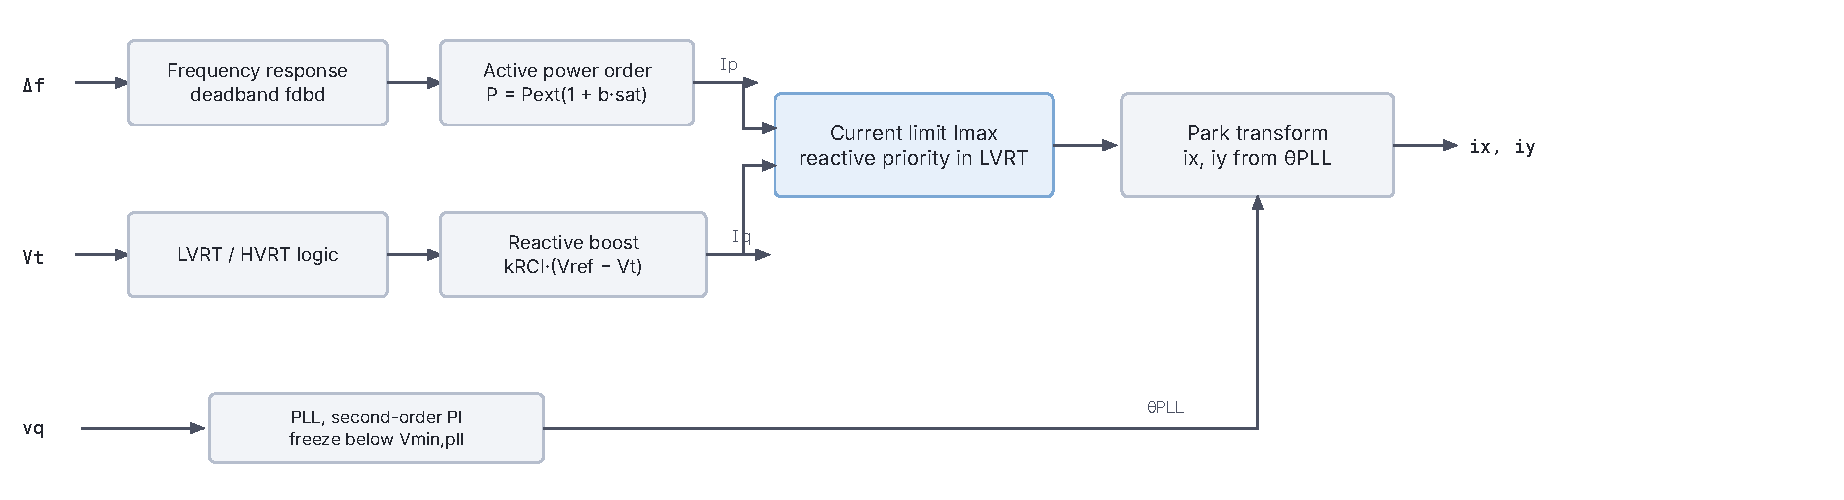
\includegraphics[width=0.98\linewidth]{figures/inj-ibg-light}
\caption{Generic inverter-based generator block diagram.}
\end{figure}

\subsubsection{Scientific Description}\label{model-inj:scientific-description-8}

The PLL tracks the terminal voltage angle \(\theta\) via a second-order PI controller with a freeze option below \(V_{\mathrm{min,pll}}\):

\[\frac{d\theta_{\mathrm{PLL}}}{dt} = \Delta\omega_{\mathrm{PLL}}, \qquad \frac{d\Delta\omega_{\mathrm{PLL}}}{dt} = k_{\mathrm{PLL}}\, v_q\]

where \(v_q\) is the \(q\)-axis terminal voltage in the PLL frame. The current commands \(I_{p,\mathrm{cmd}}\) and \(I_{q,\mathrm{cmd}}\) are derived from outer controls:

\begin{itemize}
\item
  Active power is modulated by frequency according to frequency deadband \texttt{fdbd}:
  \[P = P_{\mathrm{ext}}\left(1 + b\,\mathrm{sat}(\Delta f - f_{\mathrm{start}}, f_{\mathrm{min}}, f_{\mathrm{max}})\right)\]
\item
  During voltage dips (LVRT), reactive current is boosted:
  \[I_{q,\mathrm{boost}} = k_{\mathrm{RCI}}\,(V_{\mathrm{ref}} - V_t)\]
\item
  Current magnitude is limited to \(I_{\mathrm{max}}\) with priority to reactive current during LVRT.
\end{itemize}

The injected currents in \(x\)-\(y\) frame are:

\[i_x = I_p \cos\theta_{\mathrm{PLL}} - I_q \sin\theta_{\mathrm{PLL}}\]
\[i_y = I_p \sin\theta_{\mathrm{PLL}} + I_q \cos\theta_{\mathrm{PLL}}\]

\subsubsection{Parameters}\label{model-inj:parameters-8}

\begin{small}\begin{longtable}[]{@{}llll@{}}
\toprule\noalign{}
\# & Name & Description & Unit \\
\midrule\noalign{}
\endhead
\bottomrule\noalign{}
\endlastfoot
1 & \texttt{Imax} & Maximum current magnitude & pu \\
2 & \texttt{IN} & Nominal current & pu \\
3 & \texttt{Iprate} & Active current ramp rate & pu/s \\
4 & \texttt{Tg} & Generator time constant & s \\
5 & \texttt{Tm} & Measurement filter time constant & s \\
6 & \texttt{tLVRT1} & LVRT ride-through time threshold 1 & s \\
7 & \texttt{tLVRT2} & LVRT ride-through time threshold 2 & s \\
8 & \texttt{tLVRTint} & LVRT integration time & s \\
9 & \texttt{Vmax} & Maximum voltage for operation & pu \\
10 & \texttt{tau} & PLL response time & ms \\
11 & \texttt{Vminpll} & Voltage below which PLL is frozen & pu \\
12 & \texttt{a} & LVRT voltage-current curve slope & \\
13 & \texttt{Vmin} & Minimum LVRT voltage & pu \\
14 & \texttt{Vint} & Intermediate LVRT voltage & pu \\
15 & \texttt{fmin} & Minimum frequency for operation & pu \\
16 & \texttt{fmax} & Maximum frequency for operation & pu \\
17 & \texttt{fstart} & Frequency threshold for P modulation & pu \\
18 & \texttt{b} & Frequency droop gain & \\
19 & \texttt{fr} & Reference frequency & pu \\
20 & \texttt{Tr} & Reconnection delay after trip & s \\
21 & \texttt{Re} & Grid equivalent resistance & pu \\
22 & \texttt{Xe} & Grid equivalent reactance & pu \\
23 & \texttt{CM1} & LVRT control mode flag & \\
24 & \texttt{kRCI} & Reactive current injection gain (LVRT) & \\
25 & \texttt{kRCA} & Reactive current absorption gain (HVRT) & \\
26 & \texttt{m} & Active-reactive current priority parameter & \\
27 & \texttt{n} & Active-reactive current priority parameter & \\
28 & \texttt{dbmin} & Frequency deadband lower limit & pu \\
29 & \texttt{dbmax} & Frequency deadband upper limit & pu \\
30 & \texttt{HVRT} & HVRT flag & \\
31 & \texttt{LVRT} & LVRT flag & \\
32 & \texttt{CM2} & Control mode 2 flag & \\
33 & \texttt{Vtrip} & Trip voltage threshold & pu \\
\end{longtable}\end{small}

\subsubsection{State Variables}\label{model-inj:state-variables-8}

\begin{small}\begin{longtable}[]{@{}ll@{}}
\toprule\noalign{}
Variable & Description \\
\midrule\noalign{}
\endhead
\bottomrule\noalign{}
\endlastfoot
\texttt{vxl}, \texttt{vyl} & Filtered terminal voltage components \\
\texttt{Vt} & Terminal voltage magnitude \\
\texttt{PLLPhaseAngle} & PLL phase angle \\
\texttt{Vm} & Voltage magnitude measurement \\
\texttt{Ip}, \texttt{Iq} & Active and reactive current outputs \\
\texttt{Ipcmd}, \texttt{Iqcmd} & Current commands \\
\texttt{Iqmax}, \texttt{Iqmin} & Reactive current limits \\
\texttt{Ipmax}, \texttt{Ipmin} & Active current limits \\
\texttt{DeltaW}, \texttt{DeltaWf} & Frequency deviation and filtered value \\
\texttt{Pgen}, \texttt{Qgen} & Generated active and reactive power \\
\end{longtable}\end{small}

\subsubsection{Usage Example}\label{model-inj:usage-example-8}

\begin{Verbatim}
INJEC  IBG  IBG1  BUS_GEN  1.  1.  0.  0.  1.2  1.0  0.5  0.02  0.01  0.5  1.0  0.05
                            1.1  20.0  0.1  2.0  0.1  0.5  0.95  1.05
                            0.0  2.0  1.0  1.0  0.0  0.05  1  2.0  1.5
                            2.0  2.0  -0.02  0.02  1  1  1  0.85  ;
\end{Verbatim}

\begin{center}\rule{0.5\linewidth}{0.5pt}\end{center}

\subsection{\texorpdfstring{WT3 (\texttt{inj\_WT3}): Type 3 Wind Turbine (DFIG)}{WT3 (inj\_WT3): Type 3 Wind Turbine (DFIG)}}\label{model-inj:wt3-inj_wt3-type-3-wind-turbine-dfig}

The data-file model name is \texttt{WT3} (or \texttt{inj\_WT3}).

\subsubsection{Description}\label{model-inj:description-9}

A Type 3 wind turbine model implementing the WECC composite structure with four coupled sub-models:
- \textbf{REPC\_A}: Plant-level controller (reactive power / voltage regulation, frequency response)
- \textbf{REEC\_A}: Electrical controller (inner \(d\)-\(q\) current control, LVRT/HVRT logic)
- \textbf{WTGTRQ\_A}: Generator torque controller (rotor speed regulation via electrical torque command)
- \textbf{WTGPT\_A}: Pitch controller (aerodynamic power limitation)
- \textbf{WTGAR\_A}: Aerodynamic rotor model
- \textbf{WTGT\_A}: Two-mass mechanical drivetrain (turbine inertia \(H_t\), generator inertia \(H_g\), shaft stiffness \(K_{\mathrm{shaft}}\), damping \(D_{\mathrm{shaft}}\))

The doubly-fed induction generator (DFIG) topology allows decoupled control of active and reactive power via rotor-side converter injection.

\begin{figure}[htbp]
\centering
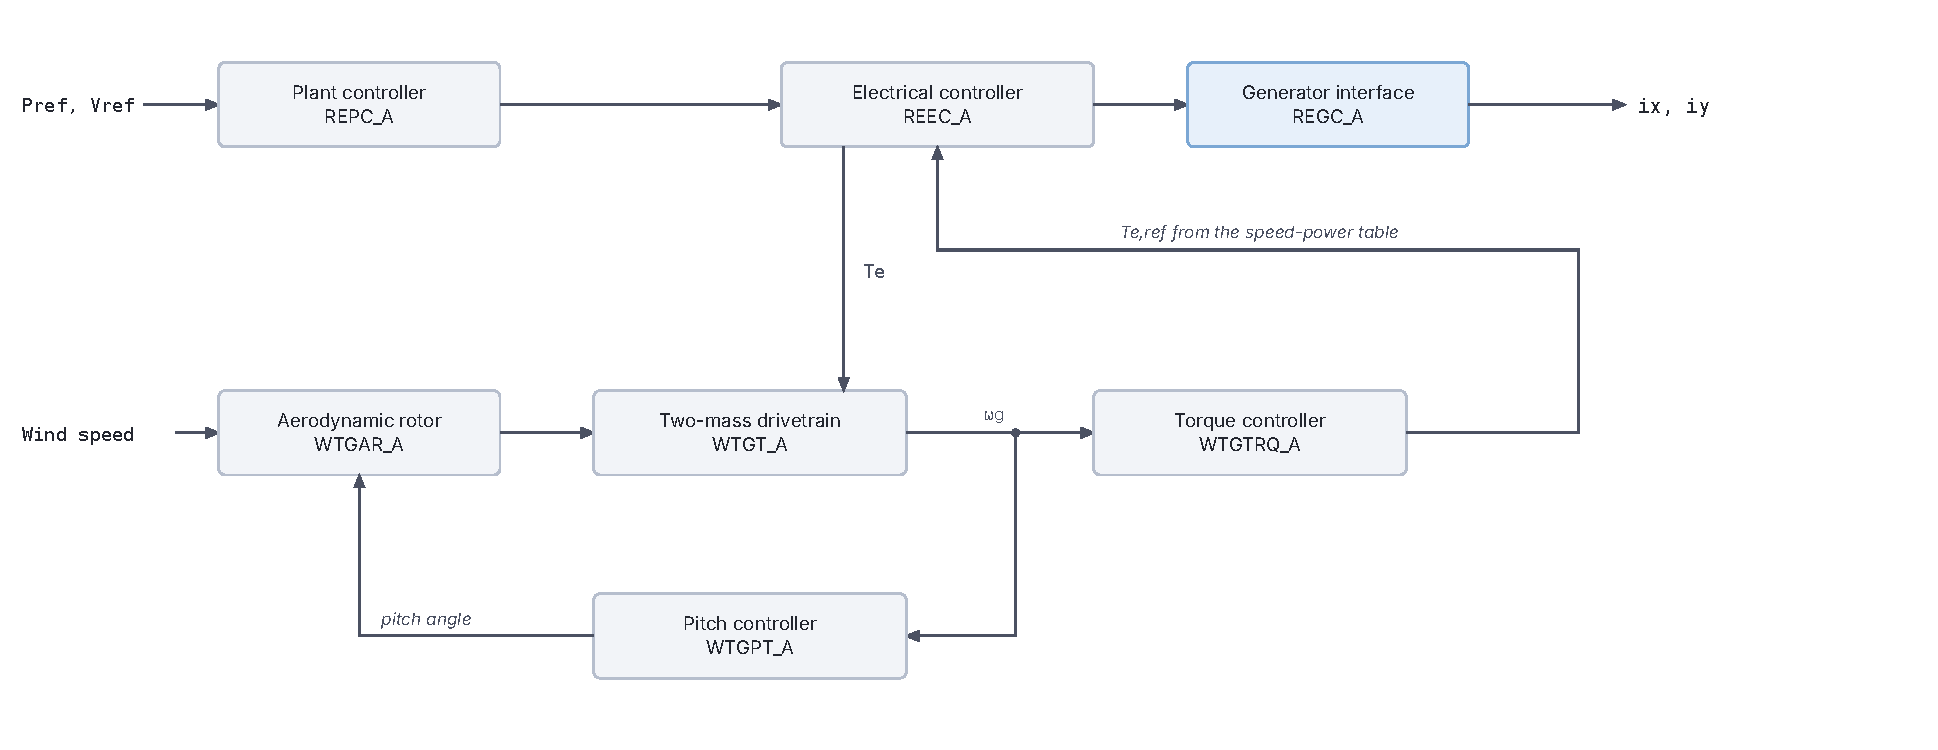
\includegraphics[width=0.98\linewidth]{figures/inj-wt3-light}
\caption{WT3 block diagram.}
\end{figure}

\subsubsection{Scientific Description}\label{model-inj:scientific-description-9}

The two-mass drivetrain model governs rotor dynamics:

\[2H_t \frac{d\omega_t}{dt} = T_m - K_{\mathrm{shaft}}(\theta_t - \theta_g) - D_{\mathrm{shaft}}(\omega_t - \omega_g)\]

\[2H_g \frac{d\omega_g}{dt} = K_{\mathrm{shaft}}(\theta_t - \theta_g) + D_{\mathrm{shaft}}(\omega_t - \omega_g) - T_e\]

The torque controller (WTGTRQ\_A) uses a piecewise power-speed characteristic:

\[T_{e,\mathrm{ref}} = \mathrm{interp}(\omega_g;\; [(\mathrm{spd}_1, p_1), (\mathrm{spd}_2, p_2), (\mathrm{spd}_3, p_3), (\mathrm{spd}_4, p_4)])\]

The electrical controller (REEC\_A) provides reactive current injection during voltage dips:

\[I_{q,\mathrm{vdip}} = k_{qv}\left(V_{\mathrm{ref0}} - V_t\right)\quad \text{when } V_t < V_{\mathrm{dip}}\]

with limiter \([I_{ql1}, I_{qh1}]\).

The plant controller (REPC\_A) optionally provides frequency response:

\[\Delta P_{\mathrm{ref}} = D_{\mathrm{dn}}\,\mathrm{sat}(\Delta f, f_{\mathrm{dbd1}}, 0) + D_{\mathrm{up}}\,\mathrm{sat}(\Delta f, 0, f_{\mathrm{dbd2}})\]

\textbf{Network interface.} REGC\_A injects a current rather than a voltage behind an
impedance. The filtered active and reactive current commands \(I_{pf}\), \(I_{qf}\) are
resolved into the network frame with the PLL angle and rescaled from the machine
rating to the system base:

\[i_x = \left(I_{pf}\cos\theta_{\mathrm{pll}} + I_{qf}\sin\theta_{\mathrm{pll}}\right)\frac{S_{\mathrm{nom}}}{S_{\mathrm{base}}}\]

\[i_y = \left(I_{pf}\sin\theta_{\mathrm{pll}} - I_{qf}\cos\theta_{\mathrm{pll}}\right)\frac{S_{\mathrm{nom}}}{S_{\mathrm{base}}}\]

The PLL angle itself tracks the \(q\)-axis component of the filtered terminal voltage:

\[v_q = -v_{x,\mathrm{filt}}\sin\theta_{\mathrm{pll}} + v_{y,\mathrm{filt}}\cos\theta_{\mathrm{pll}}\]

\hyperref[model-inj:wt4-inj_wt4-type-4-wind-turbine-full-converter]{WT4} and
\hyperref[model-inj:bess-inj_bess-battery-energy-storage-system]{BESS} use the same interface.

\subsubsection{Parameters (selected key parameters)}\label{model-inj:parameters-selected-key-parameters}

\begin{small}\begin{longtable}[]{@{}
  >{\raggedright\arraybackslash}p{(\linewidth - 10\tabcolsep) * \real{0.1380}}
  >{\raggedright\arraybackslash}p{(\linewidth - 10\tabcolsep) * \real{0.1603}}
  >{\raggedright\arraybackslash}p{(\linewidth - 10\tabcolsep) * \real{0.1927}}
  >{\raggedright\arraybackslash}p{(\linewidth - 10\tabcolsep) * \real{0.3611}}
  >{\raggedright\arraybackslash}p{(\linewidth - 10\tabcolsep) * \real{0.1480}}
@{}}
\toprule\noalign{}
\begin{minipage}[b]{\linewidth}\raggedright
\#
\end{minipage} & \begin{minipage}[b]{\linewidth}\raggedright
Name
\end{minipage} & \begin{minipage}[b]{\linewidth}\raggedright
Sub-model
\end{minipage} & \begin{minipage}[b]{\linewidth}\raggedright
Description
\end{minipage} & \begin{minipage}[b]{\linewidth}\raggedright
Unit
\end{minipage} \\
\midrule\noalign{}
\endhead
\bottomrule\noalign{}
\endlastfoot
1 & \texttt{SNOM} & & Nominal power & MW \\
2--32 & REPC\_A & Plant controller & Reactive/voltage/frequency control & various \\
33--46 & WTGTRQ\_A & Torque ctrl & Speed-torque lookup table, rate limits & various \\
47--56 & WTGPT\_A & Pitch ctrl & Pitch PI gains, angle limits, rate limits & various \\
57--58 & WTGAR\_A & Aero & Aerodynamic gain, initial pitch angle & \\
59--62 & WTGT\_A & Drivetrain & \(H_t\), \(H_g\), \(D_{\mathrm{shaft}}\), \(K_{\mathrm{shaft}}\) & s, pu \\
63--97 & REEC\_A & Elec ctrl & LVRT/HVRT, current limits, inner PI & various \\
98+ & REGC\_A & Generator & Generator electrical conversion & various \\
\end{longtable}\end{small}

Full parameter list has 80+ entries; refer to a working example data file for the complete ordering.

\subsubsection{Usage Example}\label{model-inj:usage-example-9}

\begin{Verbatim}
INJEC  WT3  WT3_1  BUS_WIND  1.  1.  0.  0.
    100.0  0.0  0.02  0  0.0  0.05  0  0.0  0.3  -0.3  2.0  0.4  0.3  -0.3  0.0  0.15  0.9  0.05
    0.0  -0.06  0.06  -0.05  0.05  0.05  -0.05  2.0  1.0  1.0  -1.0  0.02  0  0  0.8
    1.5  1.5  0.01  0.5  ... ;
\end{Verbatim}

\begin{center}\rule{0.5\linewidth}{0.5pt}\end{center}

\subsection{\texorpdfstring{WT4 (\texttt{inj\_WT4}): Type 4 Wind Turbine (Full Converter)}{WT4 (inj\_WT4): Type 4 Wind Turbine (Full Converter)}}\label{model-inj:wt4-inj_wt4-type-4-wind-turbine-full-converter}

The data-file model name is \texttt{WT4} (or \texttt{inj\_WT4}).

\subsubsection{Description}\label{model-inj:description-10}

A Type 4 wind turbine with full-rated converter. Unlike Type 3, the generator is fully decoupled from the grid through a back-to-back converter. The model implements the same WECC framework as WT3 but without the doubly-fed rotor circuit: the mechanical sub-model is a single-mass (or two-mass) drive train, and all electrical power passes through the converter. Sub-models include REPC\_A (plant controller), REEC\_A (electrical controller), WTGT\_A (drivetrain), and REGC\_A (generator/converter).

\begin{figure}[htbp]
\centering
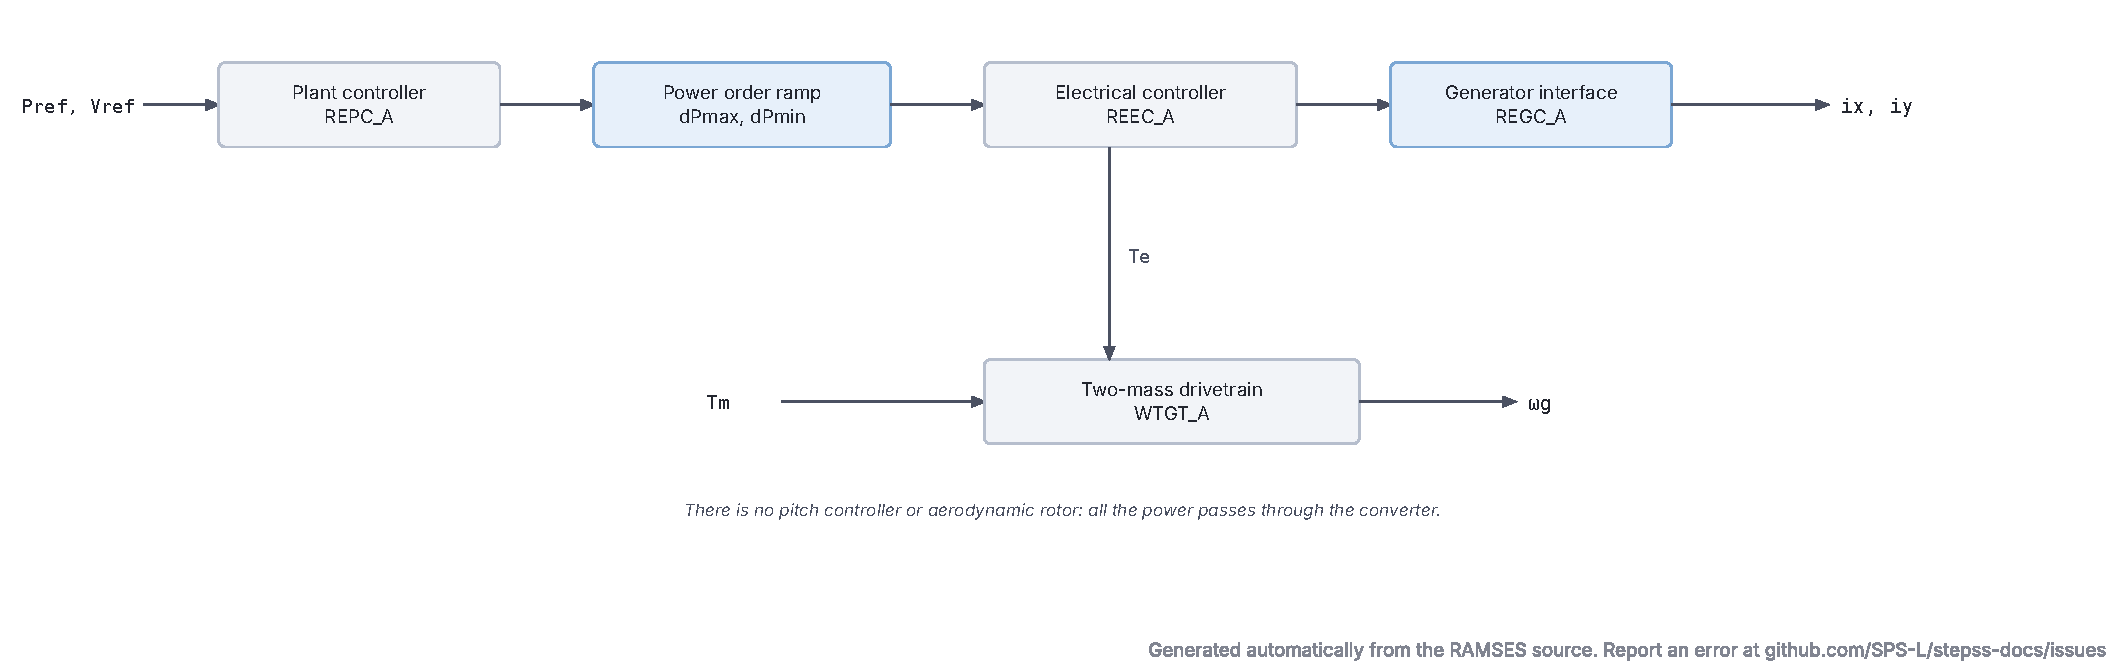
\includegraphics[width=0.98\linewidth]{figures/inj-wt4-light}
\caption{WT4 block diagram.}
\end{figure}

\subsubsection{Scientific Description}\label{model-inj:scientific-description-10}

The two-mass drivetrain is identical to WT3:

\[2H_t \frac{d\omega_t}{dt} = T_m - K_{\mathrm{shaft}}\delta_{\mathrm{shaft}} - D_{\mathrm{shaft}}(\omega_t - \omega_g)\]

\[2H_g \frac{d\omega_g}{dt} = K_{\mathrm{shaft}}\delta_{\mathrm{shaft}} + D_{\mathrm{shaft}}(\omega_t - \omega_g) - T_e\]

\[\frac{d\delta_{\mathrm{shaft}}}{dt} = \omega_0(\omega_t - \omega_g)\]

There is no pitch controller or aerodynamic rotor in the basic Type 4 configuration; the active power reference is supplied directly (or from REPC\_A), and rate limits \texttt{dPmax}/\texttt{dPmin} apply to the power order ramp.

The REEC\_A electrical controller supplies current commands with the same LVRT/HVRT logic as WT3, with current limits through the converter lookup table (piecewise linear in voltage: \((V_{p1}, I_{p1}),\ldots,(V_{p4}, I_{p4})\) for active current and \((V_{q1}, I_{q1}),\ldots,(V_{q4}, I_{q4})\) for reactive).

\subsubsection{Parameters (selected key parameters)}\label{model-inj:parameters-selected-key-parameters-1}

\begin{small}\begin{longtable}[]{@{}
  >{\raggedright\arraybackslash}p{(\linewidth - 10\tabcolsep) * \real{0.1367}}
  >{\raggedright\arraybackslash}p{(\linewidth - 10\tabcolsep) * \real{0.1649}}
  >{\raggedright\arraybackslash}p{(\linewidth - 10\tabcolsep) * \real{0.1998}}
  >{\raggedright\arraybackslash}p{(\linewidth - 10\tabcolsep) * \real{0.3336}}
  >{\raggedright\arraybackslash}p{(\linewidth - 10\tabcolsep) * \real{0.1649}}
@{}}
\toprule\noalign{}
\begin{minipage}[b]{\linewidth}\raggedright
\#
\end{minipage} & \begin{minipage}[b]{\linewidth}\raggedright
Name
\end{minipage} & \begin{minipage}[b]{\linewidth}\raggedright
Sub-model
\end{minipage} & \begin{minipage}[b]{\linewidth}\raggedright
Description
\end{minipage} & \begin{minipage}[b]{\linewidth}\raggedright
Unit
\end{minipage} \\
\midrule\noalign{}
\endhead
\bottomrule\noalign{}
\endlastfoot
1 & \texttt{SNOM} & & Nominal power & MW \\
2--32 & REPC\_A & Plant ctrl & Same as WT3 & various \\
33--37 & WTGT\_A & Drivetrain & \(H_t\), \(H_g\), \(\omega_0\), \(D_{\mathrm{shaft}}\), \(K_{\mathrm{shaft}}\) & s, pu \\
38--80 & REEC\_A & Elec ctrl & LVRT, current limits, PI gains & various \\
81+ & REGC\_A & Generator & Converter electrical model & various \\
\end{longtable}\end{small}

\subsubsection{Usage Example}\label{model-inj:usage-example-10}

\begin{Verbatim}
INJEC  WT4  WT4_1  BUS_WIND  1.  1.  0.  0.
    100.0  0.0  0.02  0  0.0  0.05  0  0.0  0.3  -0.3  2.0  0.4  0.3  -0.3  0.0  0.15  0.9  0.05
    0.0  -0.06  0.06  -0.05  0.05  0.05  -0.05  2.0  1.0  1.0  -1.0  0.02  0  0  5.0  1.5  1.0  1.5  20.0  ... ;
\end{Verbatim}

\begin{center}\rule{0.5\linewidth}{0.5pt}\end{center}

\subsection{inj\_PVG: Photovoltaic Generator}\label{model-inj:inj_pvg-photovoltaic-generator}

\begin{docsnote}{Note}

Callable since 3.79. Earlier releases compiled this model under no name, so a data file referring to it was rejected. For built-in IBR modelling, use \texttt{IBG}, \texttt{WT3}, or \texttt{WT4}. Note that the subroutine inside \texttt{inj\_PVG.f90} is named \texttt{inj\_PV}; both refer to the same single model.

\end{docsnote}

\subsubsection{Description}\label{model-inj:description-11}

A photovoltaic generator model with similar WECC-derived structure to the wind turbine models. The model includes a plant controller (voltage/reactive power regulation), an electrical controller (current limits, LVRT), and generator/converter representation. Unlike wind turbines, there is no mechanical drive train; the active power set-point follows an irradiance input or a fixed reference. LVRT/HVRT logic and current limiting are identical to the Type 4 wind model.

\begin{figure}[htbp]
\centering
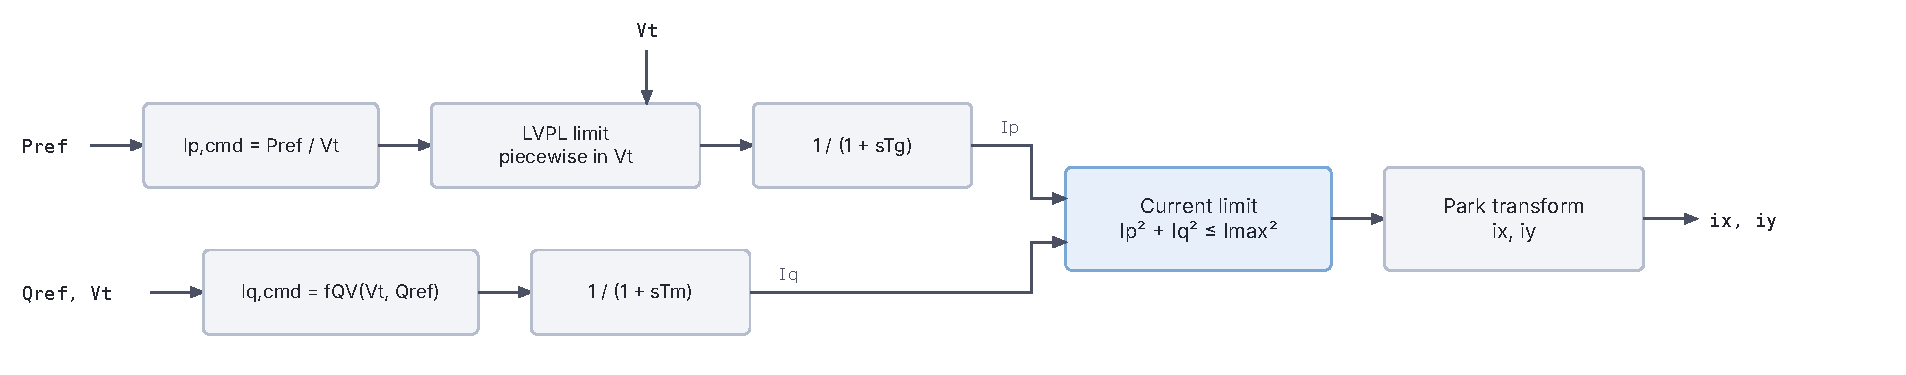
\includegraphics[width=0.98\linewidth]{figures/inj-pvg-light}
\caption{Photovoltaic generator block diagram.}
\end{figure}

\subsubsection{Scientific Description}\label{model-inj:scientific-description-11}

The PV generator delivers active and reactive power through current commands:

\[I_p = \frac{P_{\mathrm{ref}}}{V_t}, \qquad I_q = f_{\mathrm{QV}}(V_t, Q_{\mathrm{ref}})\]

subject to the constraint \(\sqrt{I_p^2 + I_q^2} \leq I_{\mathrm{max}}\). The inner current loop is a first-order filter:

\[T_g \frac{dI_p}{dt} = I_{p,\mathrm{cmd}} - I_p, \qquad T_m \frac{dI_q}{dt} = I_{q,\mathrm{cmd}} - I_q\]

Low-voltage power-logic (LVPL) limits active current during deep voltage sags via a piecewise-linear function of \(V_t\) with breakpoints \texttt{lvpnt0}, \texttt{lvpnt1}, \texttt{Lvpl1}. HVRT and LVRT timers control disconnection and reconnection.

\subsubsection{Parameters (selected)}\label{model-inj:parameters-selected}

\begin{small}\begin{longtable}[]{@{}
  >{\raggedright\arraybackslash}p{(\linewidth - 8\tabcolsep) * \real{0.1599}}
  >{\raggedright\arraybackslash}p{(\linewidth - 8\tabcolsep) * \real{0.2391}}
  >{\raggedright\arraybackslash}p{(\linewidth - 8\tabcolsep) * \real{0.4695}}
  >{\raggedright\arraybackslash}p{(\linewidth - 8\tabcolsep) * \real{0.1315}}
@{}}
\toprule\noalign{}
\begin{minipage}[b]{\linewidth}\raggedright
\#
\end{minipage} & \begin{minipage}[b]{\linewidth}\raggedright
Name
\end{minipage} & \begin{minipage}[b]{\linewidth}\raggedright
Description
\end{minipage} & \begin{minipage}[b]{\linewidth}\raggedright
Unit
\end{minipage} \\
\midrule\noalign{}
\endhead
\bottomrule\noalign{}
\endlastfoot
1 & \texttt{Imax} & Maximum converter current & pu \\
2 & \texttt{IN} & Nominal current & pu \\
3 & \texttt{ratemax} & Reconnection ramp rate & pu/s \\
4 & \texttt{Tg} & Active current filter time constant & s \\
5 & \texttt{Tm} & Reactive current filter time constant & s \\
6--9 & LVRT timers & \texttt{tLVRT1}, \texttt{tLVRT2}, \texttt{tLVRTint}, \texttt{Vmax} & s, pu \\
10 & \texttt{kpll} & PLL gain & \\
11 & \texttt{Vminpll} & PLL freeze voltage & pu \\
12--14 & LVRT curve & \texttt{a}, \texttt{Vmin}, \texttt{Vint} & \\
21--22 & \texttt{Re}, \texttt{Xe} & Grid equivalent impedance & pu \\
23--29 & Current control & \texttt{CM1}, \texttt{kRCI}, \texttt{kRCA}, \texttt{m}, \texttt{n}, \texttt{dbmin}, \texttt{dbmax} & \\
34 & \texttt{BM} & Battery module flag & \\
\end{longtable}\end{small}

\subsubsection{Usage Example}\label{model-inj:usage-example-11}

\begin{Verbatim}
INJEC  PV  PV1  BUS_PV  1.  1.  0.  0.  1.2  1.0  0.5  0.02  0.01  0.5  1.0  0.05  1.1
                          20.0  0.1  2.0  0.1  0.5  0.95  1.05  0.0  2.0  1.0
                          1.0  0.0  0.05  1  2.0  1.5  2.0  2.0  -0.02  0.02  1  1  1  0.85  0  ;
\end{Verbatim}

\begin{center}\rule{0.5\linewidth}{0.5pt}\end{center}

\subsection{\texorpdfstring{GFOR (\texttt{inj\_GFOR}): Grid-Forming Converter (VSM)}{GFOR (inj\_GFOR): Grid-Forming Converter (VSM)}}\label{model-inj:gfor-inj_gfor-grid-forming-converter-vsm}

The data-file model name is \texttt{GFOR} (or \texttt{inj\_GFOR}).

\subsubsection{Description}\label{model-inj:description-12}

A grid-forming voltage source converter implementing Virtual Synchronous Machine (VSM) dynamics, modelled under the phasor approximation. The converter is an MMC-type VSC connected to the grid through its transformer (no LC filter); the DC side is not modelled (the DC voltage is assumed constant) so the focus is on the AC grid dynamics.

The modulated voltage magnitude is held at its setpoint \(V_m^0\) in normal operation, while the phase angle \(\delta_m\) is driven by a synthetic swing equation with inertia emulation (\(H\)) and oscillation damping (\(D\)) against a PLL estimate of the grid frequency. Participation in primary frequency control is optional, through the droop \(R_{\mathrm{droop}}\). Overcurrents are limited by proportionally scaling the \(d\)-\(q\) current vector back to the \(I_{\mathrm{max}}\) circle with a small time constant.

\subsubsection{Scientific Description}\label{model-inj:scientific-description-12}

\textbf{Reference frame.} The \(d\) axis is attached to the internal phase angle \(\delta_m\) of the modulated voltage. Voltages and currents at the point of common coupling are transformed as:

\[v_d = v_x\cos\delta_m + v_y\sin\delta_m, \qquad v_q = -v_x\sin\delta_m + v_y\cos\delta_m\]

with the analogous transformation for the converter-side currents \(i_{xt} = k\, i_x\), \(i_{yt} = k\, i_y\), where \(k = r\, S_{\mathrm{base}}/S_{\mathrm{nom}}\) converts to per-unit on the converter base.

\textbf{Transformer.} The voltage-current relationship across the connection transformer (resistance \(R\), inductance \(L\), ideal ratio \(r\)) in the \(d\)-\(q\) frame is:

\[v_{md} = \frac{v_d}{r} + R\, i_d - \omega_m L\, i_q, \qquad v_{mq} = \frac{v_q}{r} + R\, i_q + \omega_m L\, i_d\]

\textbf{PLL.} The PLL only serves to estimate the grid angular frequency \(\tilde{\omega}_g\) for the damping term. It is the same model as in the grid-following converter (see the \hyperref[model-inj:gfol-inj_gfol-grid-following-converter]{PLL diagram there}), with PI gains derived from the time constant \(T_{\mathrm{pll}}\):

\[K_{p\omega} = \frac{10}{\omega_N T_{\mathrm{pll}}}, \qquad K_{i\omega} = \frac{25}{\omega_N T_{\mathrm{pll}}^2}, \qquad \omega_N = 2\pi f_N\]

The PLL is frozen (hysteresis) when the PCC voltage falls below 0.4 pu and reactivated when it recovers above 0.5 pu (fixed thresholds in this model).

\textbf{Active power and phase angle control (VSM).}

\begin{figure}[htbp]
\centering
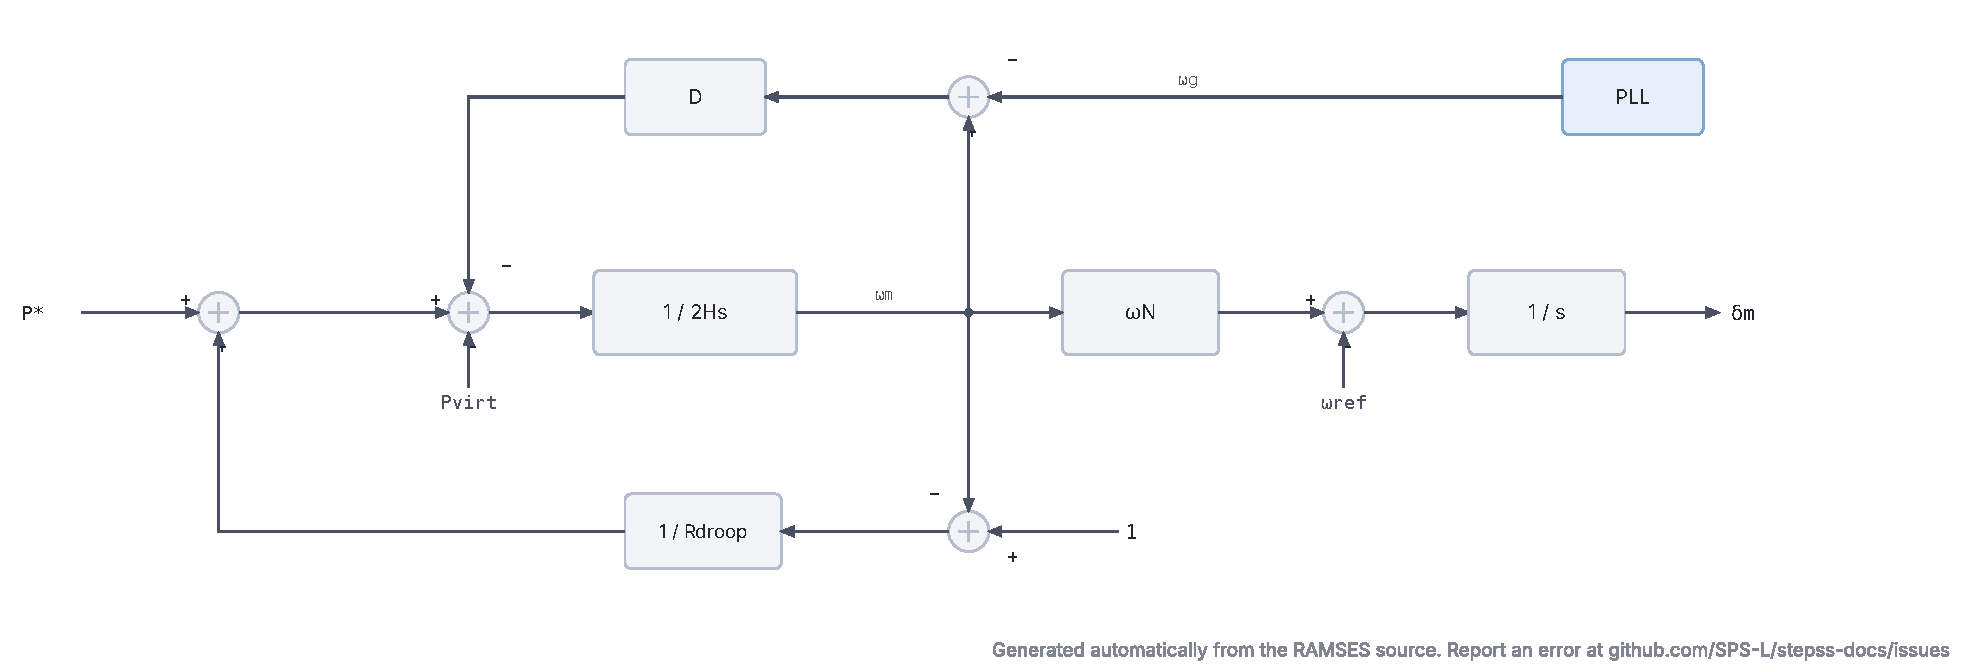
\includegraphics[width=0.98\linewidth]{figures/inj-gfor-vsm-light}
\caption{Grid-forming virtual synchronous machine block diagram.}
\end{figure}

\[2H\frac{d\omega_m}{dt} = P^* - P_{\mathrm{virt}} - D\left(\omega_m - \tilde{\omega}_g\right) + \frac{1 - \omega_m}{R_{\mathrm{droop}}}\]

\[\frac{d\delta_m}{dt} = \omega_N\left(\omega_m - \omega_{\mathrm{ref}}\right)\]

where \(P^*\) is the active power setpoint and \(P_{\mathrm{virt}}\) is the \emph{virtual power} computed from the \textbf{unsaturated} currents:

\[P_{\mathrm{virt}} = \frac{v_d}{r}\, i_d^* + \frac{v_q}{r}\, i_q^*\]

\(P_{\mathrm{virt}}\) equals the actual active power \(P\) when the current is not limited, and yields improved large-disturbance stability while the current is limited (the angle dynamics do not wind up).

\textbf{Current limitation.} The currents \((i_d^*, i_q^*)\) that would result from normal voltage control (i.e.~\(v_{md} = V_m^0\), \(v_{mq} = 0\)) are first determined from:

\[V_m^0 = \frac{v_d}{r} + R\, i_d^* - \omega_m L\, i_q^*, \qquad 0 = \frac{v_q}{r} + R\, i_q^* + \omega_m L\, i_d^*\]

The current overload ratio \(\rho = \sqrt{(i_d^*)^2 + (i_q^*)^2}\,/\,I_{\mathrm{max}}\) is passed through a first-order lag with time constant \(T_e\) (typically 1 ms) and a non-windup \textbf{lower limit of 1}, giving \(\rho_s\). Both current components are then decreased in the same proportion:

\[i_{ds}^* = \frac{i_d^*}{\rho_s}, \qquad i_{qs}^* = \frac{i_q^*}{\rho_s}\]

\begin{figure}[htbp]
\centering
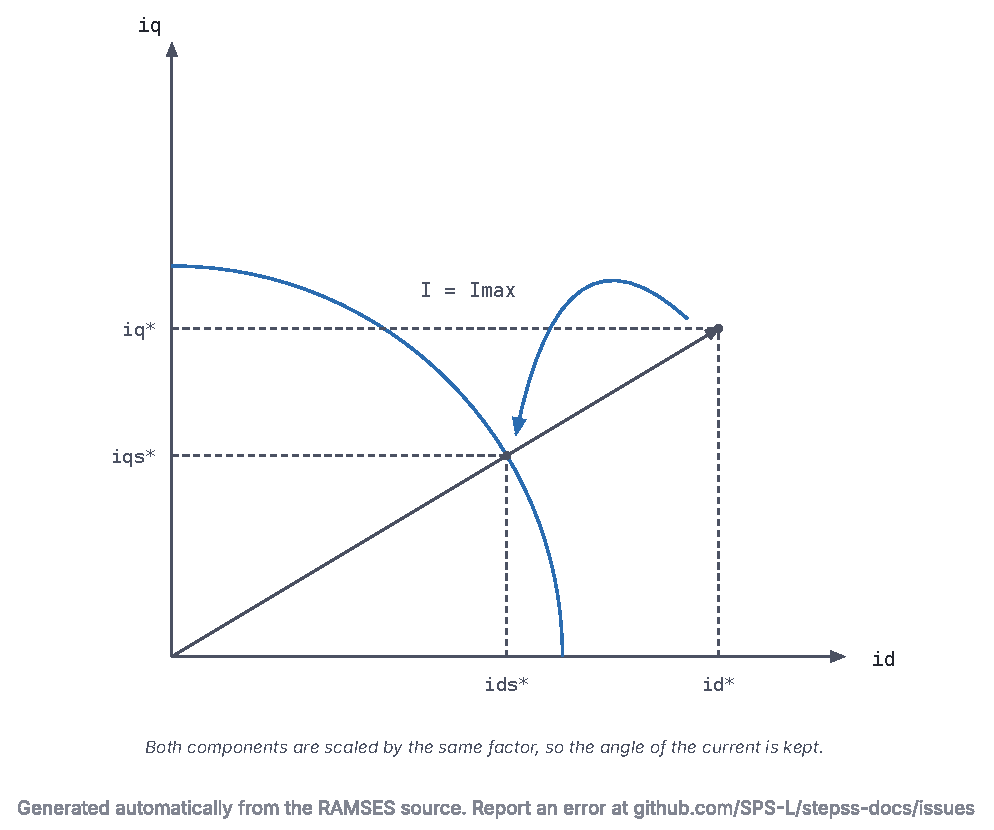
\includegraphics[width=0.98\linewidth]{figures/inj-gfor-currentlim-light}
\caption{Grid-forming current limitation.}
\end{figure}

and the modulated voltage is set to the value that yields the saturated currents:

\[v_{md} = \frac{v_d}{r} + R\, i_{ds}^* - \omega_m L\, i_{qs}^*, \qquad v_{mq} = \frac{v_q}{r} + R\, i_{qs}^* + \omega_m L\, i_{ds}^*\]

When \(I < I_{\mathrm{max}}\): \(\rho_s = 1\), the currents are unsaturated, and \(v_{md} = V_m^0\), \(v_{mq} = 0\).

\subsubsection{Parameters}\label{model-inj:parameters-9}

Default values correspond to a 1100 MVA converter. Per-unit values refer to the nominal apparent power of the converter.

\begin{small}\begin{longtable}[]{@{}lllll@{}}
\toprule\noalign{}
\# & Name & Description & Unit & Default \\
\midrule\noalign{}
\endhead
\bottomrule\noalign{}
\endlastfoot
1 & \texttt{R} & Resistance of connection transformer & pu & 0.005 \\
2 & \texttt{L} & Inductance of connection transformer & pu & 0.15 \\
3 & \texttt{r} & Ratio of ideal transformer & & 1.02 \\
4 & \texttt{Snom} & Nominal apparent power & MVA & 1100 \\
5 & \texttt{H} & Inertia constant & s & 5.0 \\
6 & \texttt{D} & Damping constant of virtual synchronous machine & & 300 \\
7 & \texttt{Tpll} & Time constant of PLL & s & 0.1 \\
8 & \texttt{Rdroop} & Droop of primary frequency control & pu & 999 \\
9 & \texttt{Imax} & Maximum current (typically 1--1.2) & pu & 1.0 \\
10 & \texttt{Te} & Time constant of current saturation & s & 0.001 \\
\end{longtable}\end{small}

A very large \texttt{Rdroop} (e.g.~999) effectively disables participation in primary frequency control.

Five additional parameters are computed at initialization from the power-flow solution: \texttt{k} (current conversion factor), \texttt{vmx0}, \texttt{vmy0} (components of the initial modulated voltage), \texttt{Vmo} (its magnitude \(V_m^0\), i.e.~the voltage setpoint) and \texttt{Po} (the active power setpoint \(P^*\), pu on \texttt{Snom} base). \texttt{Vmo} and \texttt{Po} can be modified during the simulation with \texttt{CHGPRM} disturbances to change the voltage and active power setpoints.

\subsubsection{State Variables}\label{model-inj:state-variables-9}

The model has 33 states (2 output currents + 31 internal). Key internal states:

\begin{small}\begin{longtable}[]{@{}
  >{\raggedright\arraybackslash}p{(\linewidth - 6\tabcolsep) * \real{0.2782}}
  >{\raggedright\arraybackslash}p{(\linewidth - 6\tabcolsep) * \real{0.5633}}
  >{\raggedright\arraybackslash}p{(\linewidth - 6\tabcolsep) * \real{0.1585}}
@{}}
\toprule\noalign{}
\begin{minipage}[b]{\linewidth}\raggedright
Variable
\end{minipage} & \begin{minipage}[b]{\linewidth}\raggedright
Description
\end{minipage} & \begin{minipage}[b]{\linewidth}\raggedright
Unit
\end{minipage} \\
\midrule\noalign{}
\endhead
\bottomrule\noalign{}
\endlastfoot
\texttt{wref} & Angular speed of reference axes & pu \\
\texttt{ixt}, \texttt{iyt} & Converter-side currents (on \texttt{Snom} base) & pu \\
\texttt{Vm}, \texttt{deltam} & Modulated voltage magnitude and phase angle & pu, rad \\
\texttt{V} & Voltage magnitude at PCC & pu \\
\texttt{mult\_pll} & PLL freezing factor (hysteresis output) & \\
\texttt{w\_pll}, \texttt{theta\_pll} & PLL frequency and angle estimates & pu, rad \\
\texttt{P}, \texttt{Pvirt} & Active power and virtual power (on \texttt{Snom} base) & pu \\
\texttt{omegam} & Angular frequency of modulated voltage & pu \\
\texttt{vd}, \texttt{vq}, \texttt{id}, \texttt{iq} & PCC voltage and current in \(d\)-\(q\) frame & pu \\
\texttt{id*}, \texttt{iq*} & Unsaturated currents & pu \\
\texttt{id*s}, \texttt{iq*s} & Saturated currents & pu \\
\texttt{rho}, \texttt{rhos} & Current overload ratio and its saturated value & \\
\texttt{Q} & Reactive power (on \texttt{Snom} base) & pu \\
\end{longtable}\end{small}

\textbf{Observables:} \texttt{P}, \texttt{Pvirt}, \texttt{Q}, \texttt{Vm}, \texttt{vmd}, \texttt{vmq}, \texttt{deltam}, \texttt{omegam}, \texttt{w\_pll}, \texttt{I}, \texttt{id}, \texttt{id*}, \texttt{id*s}, \texttt{iq}, \texttt{iq*}, \texttt{iq*s}, \texttt{rho}, \texttt{rhos}.

\subsubsection{Usage Example}\label{model-inj:usage-example-12}

A 1100 MVA grid-forming converter:

\begin{Verbatim}
#                 name   bus  FP   FQ   P   Q    R      L     r     Snom   H     D    Tpll  Rdroop Imax   Te
INJEC    GFOR     HVDC    A   1.   1.   0.  0.  0.005  0.15  1.02  1100.  5.0   300.  0.100  999.   1.0  0.001 ;
\end{Verbatim}

\begin{docsnote}{Note}

At operating points where the initial current is below \(I_{\mathrm{max}}\), RAMSES reports a small initial mismatch on the \(\rho_s\) lag equation (``INJECTORS NOT IN STEADY STATE''). This is benign: \(\rho_s\) starts exactly at its lower limit of 1 and is clamped there by the discrete update within the first time step.

\end{docsnote}

\begin{center}\rule{0.5\linewidth}{0.5pt}\end{center}

\subsection{\texorpdfstring{GFOL (\texttt{inj\_GFOL}): Grid-Following Converter}{GFOL (inj\_GFOL): Grid-Following Converter}}\label{model-inj:gfol-inj_gfol-grid-following-converter}

The data-file model name is \texttt{GFOL} (or \texttt{inj\_GFOL}).

\subsubsection{Description}\label{model-inj:description-13}

A grid-following voltage source converter modelled under the phasor approximation. As for the grid-forming model, the converter is an MMC-type VSC connected through its transformer (no LC filter) and the DC side is not modelled. The model is rather detailed: it includes measurement low-pass filters, a PLL with blocking/unblocking hysteresis, outer active power and voltage/reactive power control loops, inner \(d\)-\(q\) current control loops, a rate-limited \(d\)-axis current limit with priority to the reactive current, and a piecewise-linear dynamic voltage support characteristic.

\subsubsection{Scientific Description}\label{model-inj:scientific-description-13}

\textbf{Reference frame.} The VSC control frame \((d, q)\) tracks the PCC voltage phasor through the PLL angle \(\tilde{\delta}_g\) (state \texttt{theta\_pll}):

\[v_d = v_x\cos\tilde{\delta}_g + v_y\sin\tilde{\delta}_g, \qquad v_q = -v_x\sin\tilde{\delta}_g + v_y\cos\tilde{\delta}_g\]

with the analogous transformation for the converter-side currents (\(i_{xt} = k\, i_x\), \(k = r\, S_{\mathrm{base}}/S_{\mathrm{nom}}\)). In steady state \(v_q = 0\) and \(v_d = V\).

\textbf{Phase Locked Loop.}

\begin{figure}[htbp]
\centering
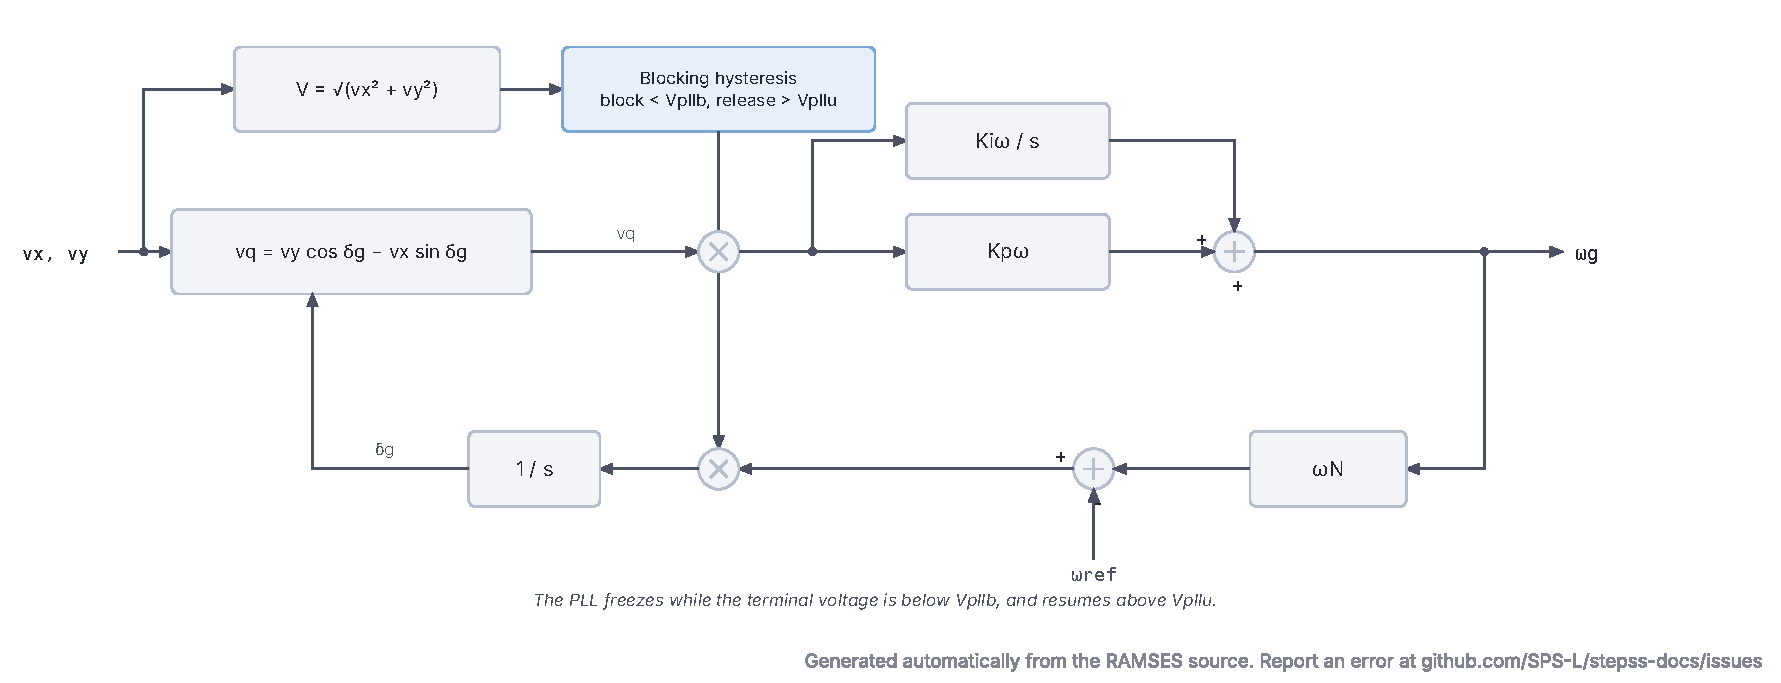
\includegraphics[width=0.98\linewidth]{figures/inj-gfol-pll-light}
\caption{Grid-following phase-locked loop block diagram.}
\end{figure}

The \(q\)-axis voltage error drives a PI controller whose output is the grid frequency estimate \(\tilde{\omega}_g\) (state \texttt{w\_pll}); integrating \(\omega_N(\tilde{\omega}_g - \omega_{\mathrm{ref}})\) gives the PLL angle. The PI gains follow from the PLL response time \(\tau\):

\[K_{p\omega} = \frac{10}{\omega_N \tau}, \qquad K_{i\omega} = \frac{25}{\omega_N \tau^2}, \qquad \omega_N = 2\pi f_N\]

The PLL is blocked once the PCC voltage \(V\) falls below \texttt{Vpllb} and reactivated once \(V\) recovers above \texttt{Vpllu} (hysteresis).

\textbf{Inner current control.}

\begin{figure}[htbp]
\centering
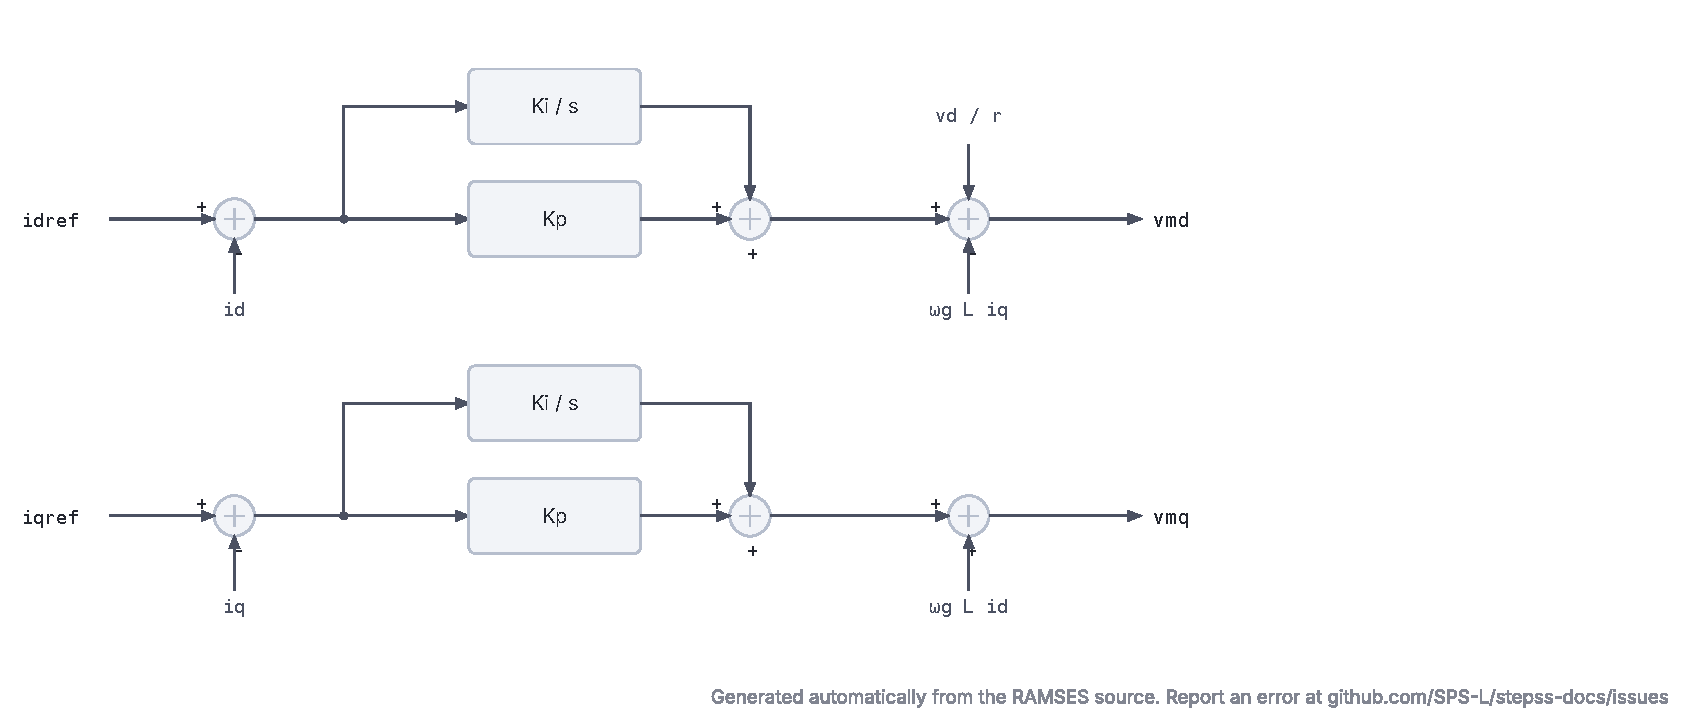
\includegraphics[width=0.98\linewidth]{figures/inj-gfol-currentctl-light}
\caption{Grid-following inner current control.}
\end{figure}

\[v_{md} = \frac{v_d}{r} - \tilde{\omega}_g L\, i_q + \left(K_p + \frac{K_i}{s}\right)\left(i_d^{\mathrm{ref}} - i_d\right)\]

\[v_{mq} = \tilde{\omega}_g L\, i_d + \left(K_p + \frac{K_i}{s}\right)\left(i_q^{\mathrm{ref}} - i_q\right)\]

combined with the transformer voltage-current relationship in the \(d\)-\(q\) frame:

\[v_{md} = \frac{v_d}{r} + R\, i_d - \tilde{\omega}_g L\, i_q, \qquad v_{mq} = \frac{v_q}{r} + R\, i_q + \tilde{\omega}_g L\, i_d\]

\textbf{Active power control.}

\begin{figure}[htbp]
\centering
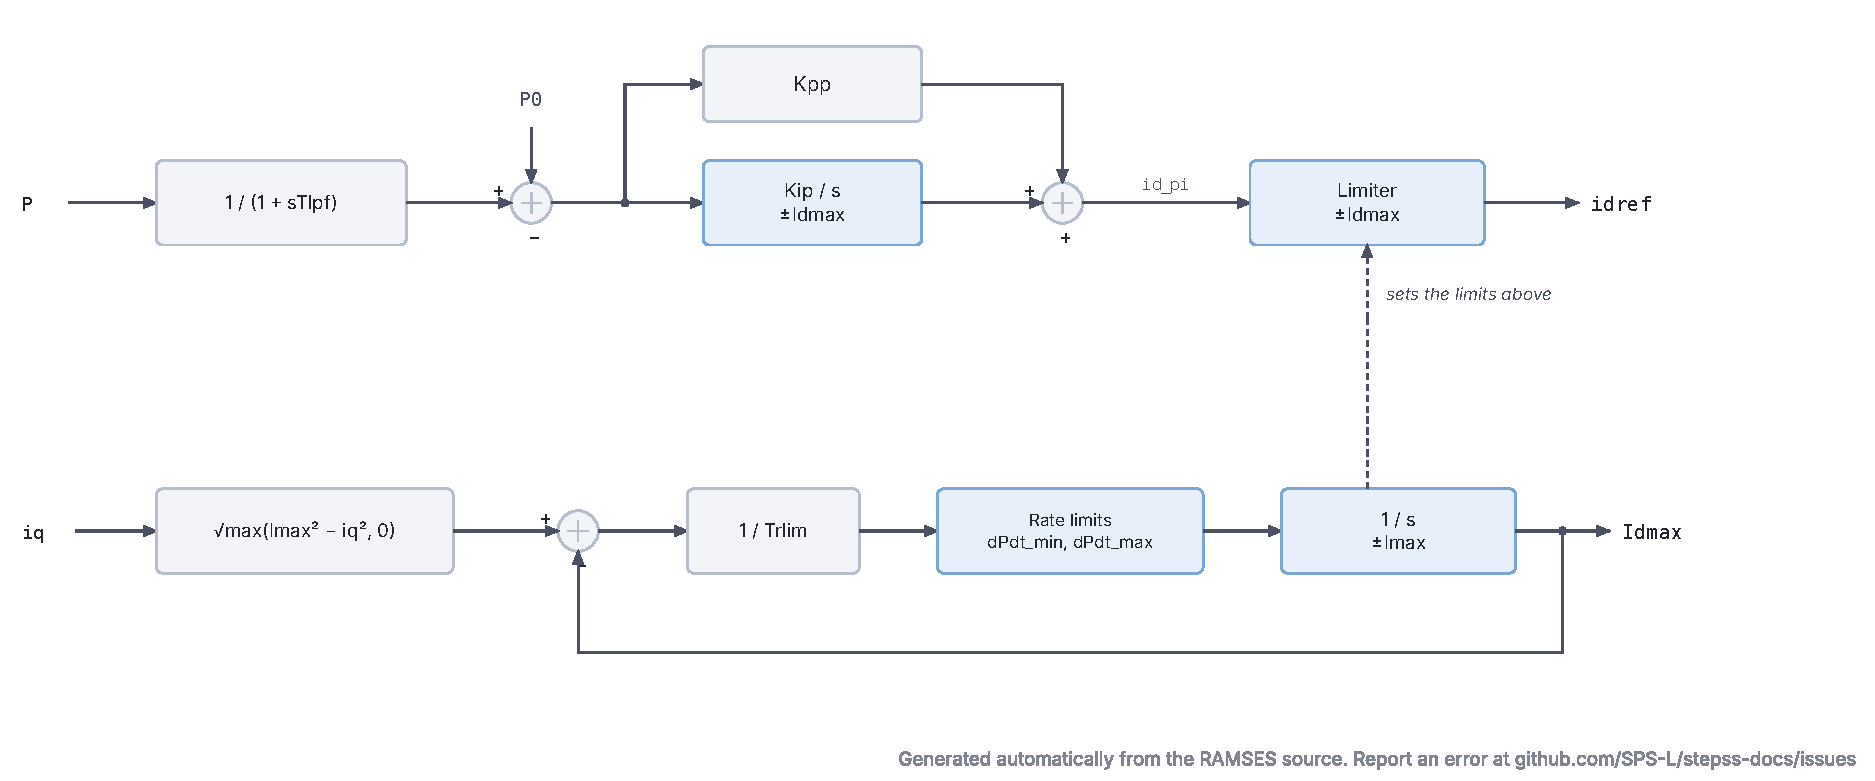
\includegraphics[width=0.98\linewidth]{figures/inj-gfol-pctl-light}
\caption{Grid-following active power control.}
\end{figure}

The measured active power is filtered with time constant \(T_{\mathrm{lpf}}\) and compared with the setpoint \(P^0\); a PI controller (\(K_{pp}\), \(K_{ip}\)) with non-windup limits \(\pm I_d^{\max}\) produces \(i_d^{\mathrm{ref}}\). The limit gives \textbf{priority to the reactive current}:

\[I_d^{\max,\mathrm{stat}} = \sqrt{\max\left(I_{\mathrm{max}}^2 - i_q^2,\; 0\right)}\]

and \(I_d^{\max}\) tracks this static value through a first-order lag (\(T_{\mathrm{rlim}}\), typically 0.002 s) with rate limits \texttt{dPdt\_min}/\texttt{dPdt\_max}, limiting in particular the rate of recovery of the active current after it has been decreased by an increase of \(i_q\).

\textbf{Voltage / reactive power control.}

\begin{figure}[htbp]
\centering
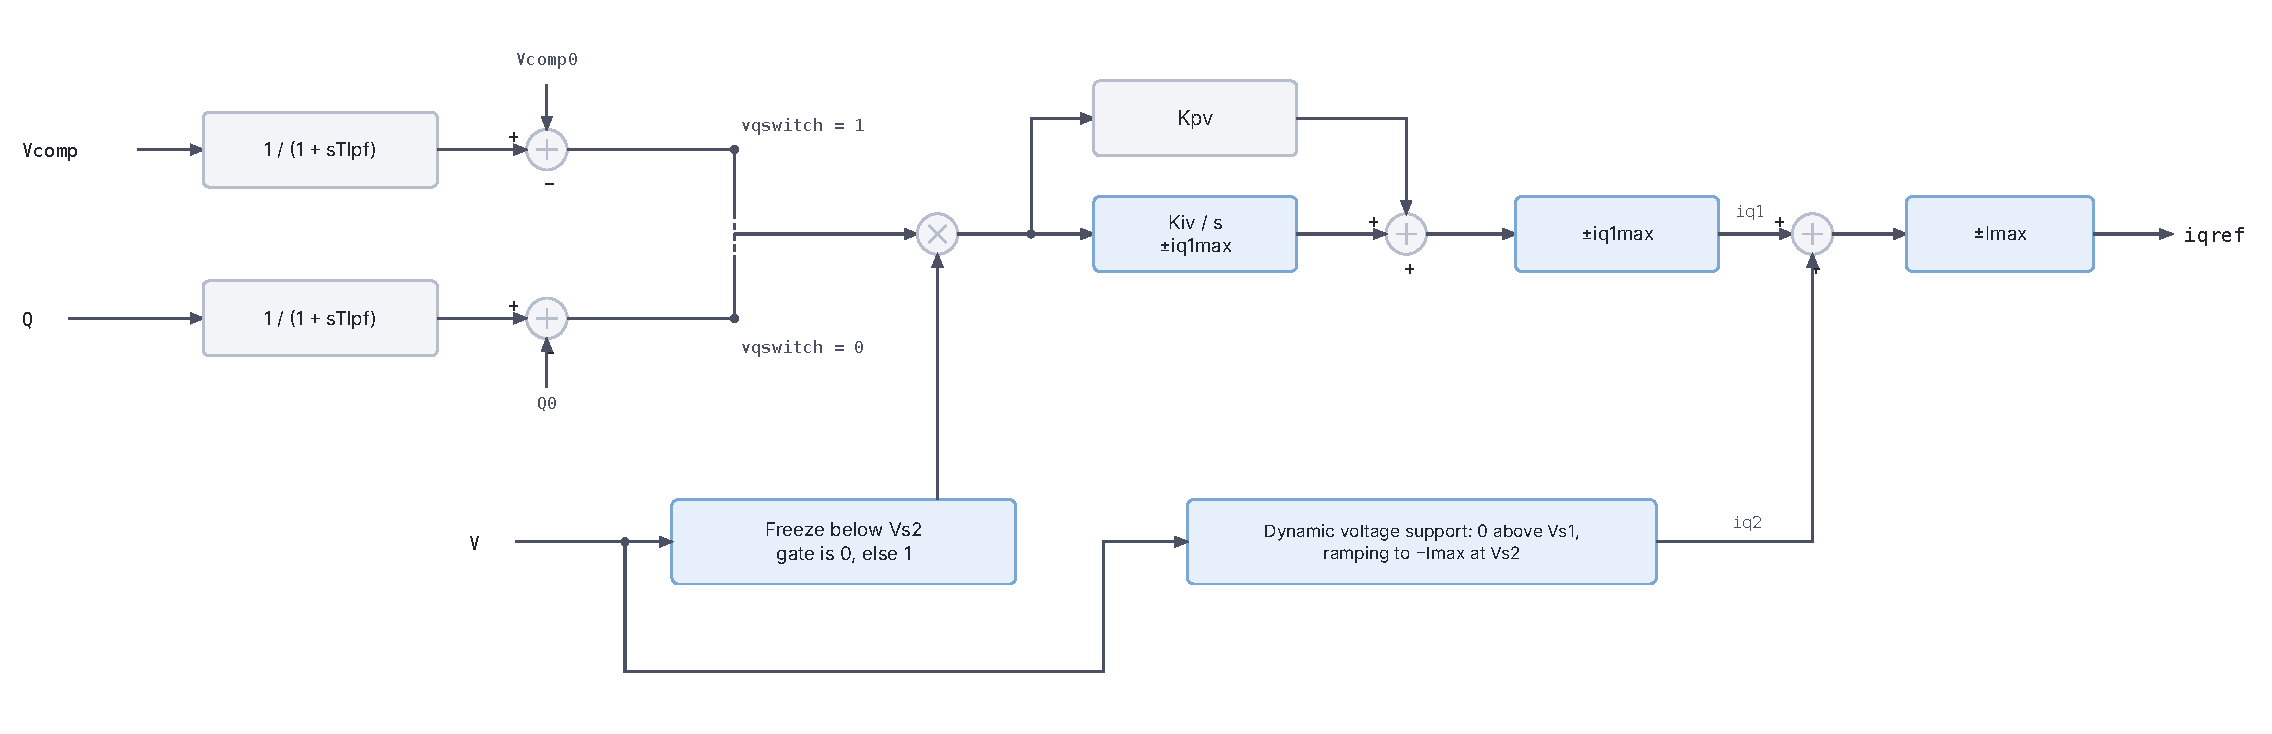
\includegraphics[width=0.98\linewidth]{figures/inj-gfol-qctl-light}
\caption{Grid-following voltage and reactive power control.}
\end{figure}

Depending on \texttt{vqswitch}, either the compensated voltage or the reactive power is controlled:

\[V_c = \left|\frac{\bar{v}}{r} + (R_c + jX_c)\,\bar{i}\right| \quad (\texttt{vqswitch}=1), \qquad Q = \frac{v_q}{r} i_d - \frac{v_d}{r} i_q \quad (\texttt{vqswitch}=0)\]

The controlled quantity is filtered (\(T_{\mathrm{lpf}}\)) and its deviation from setpoint drives a PI controller (\(K_{pv}\), \(K_{iv}\)) with non-windup limits \(\pm i_{q1}^{\max}\), giving the component \(i_{q1}\). The error is zeroed (controller frozen) while \(V < V_{s2}\). A second component \(i_{q2}\) implements dynamic voltage support as a piecewise-linear function of \(V\): zero above \(V_{s1}\), decreasing linearly to \(-I_{\mathrm{max}}\) at \(V_{s2}\), constant below. The total \(i_{q1} + i_{q2}\), limited to \(\pm I_{\mathrm{max}}\), is the reactive current reference \(i_q^{\mathrm{ref}}\).

With \(R_c = R\), \(X_c = \omega L\) and \(r = 1\), controlling \(V_c\) amounts to controlling the magnitude of the modulated voltage.

\subsubsection{Parameters}\label{model-inj:parameters-10}

Default values correspond to a 1200 MVA converter. Per-unit values refer to the nominal apparent power of the converter.

\begin{small}\begin{longtable}[]{@{}
  >{\raggedright\arraybackslash}p{(\linewidth - 10\tabcolsep) * \real{0.1005}}
  >{\raggedright\arraybackslash}p{(\linewidth - 10\tabcolsep) * \real{0.1524}}
  >{\raggedright\arraybackslash}p{(\linewidth - 10\tabcolsep) * \real{0.4781}}
  >{\raggedright\arraybackslash}p{(\linewidth - 10\tabcolsep) * \real{0.1030}}
  >{\raggedright\arraybackslash}p{(\linewidth - 10\tabcolsep) * \real{0.1659}}
@{}}
\toprule\noalign{}
\begin{minipage}[b]{\linewidth}\raggedright
\#
\end{minipage} & \begin{minipage}[b]{\linewidth}\raggedright
Name
\end{minipage} & \begin{minipage}[b]{\linewidth}\raggedright
Description
\end{minipage} & \begin{minipage}[b]{\linewidth}\raggedright
Unit
\end{minipage} & \begin{minipage}[b]{\linewidth}\raggedright
Default
\end{minipage} \\
\midrule\noalign{}
\endhead
\bottomrule\noalign{}
\endlastfoot
1 & \texttt{R} & Phase reactor resistance & pu & 0.005 \\
2 & \texttt{L} & Phase reactor inductance & pu & 0.15 \\
3 & \texttt{r} & Ratio of ideal transformer & & 1.02 \\
4 & \texttt{Snom} & Nominal apparent power & MVA & 1200 \\
5 & \texttt{Rc} & Resistance used in compensated voltage & pu & 0.005 \\
6 & \texttt{Xc} & Reactance used in compensated voltage & pu & 0.15 \\
7 & \texttt{Kp} & Current control: proportional gain & & 0.573 \\
8 & \texttt{Ki} & Current control: integral gain & & 6.0 \\
9 & \texttt{Tlpf} & Measurement time constant (low-pass filter) & s & 0.0033 \\
10 & \texttt{Kpp} & Active power control: proportional gain & & 0.0333 \\
11 & \texttt{Kip} & Active power control: integral gain & & 10.0 \\
12 & \texttt{Trlim} & Time constant of the \(I_d^{\max}\) rate limiter & s & 0.002 \\
13 & \texttt{dPdt\_min} & Min rate of change of the \(d\)-current limit & pu/s & -999 \\
14 & \texttt{dPdt\_max} & Max rate of change of the \(d\)-current limit & pu/s & 10.0 \\
15 & \texttt{Kpv} & Reactive power control: proportional gain & & 0.1667 \\
16 & \texttt{Kiv} & Reactive power control: integral gain & & 50.0 \\
17 & \texttt{tau} & Response time of PLL & s & 0.10 \\
18 & \texttt{Vpllb} & Voltage below which the PLL is blocked & pu & 0.4 \\
19 & \texttt{Vpllu} & Voltage above which the PLL is unblocked & pu & 0.5 \\
20 & \texttt{Imax} & Maximum current (typically 1--1.2) & pu & 1.0 \\
21 & \texttt{Vs1} & Voltage below which dynamic reactive support starts & pu & -1000 \\
22 & \texttt{Vs2} & Voltage at which reactive support is maximum (\(V_{s2} < V_{s1}\)) & pu & -2000 \\
23 & \texttt{iqmax} & Limit (\ensuremath{\pm}) on quadrature current component \(i_{q1}\) & pu & 1.001 \\
24 & \texttt{vqswitch} & 1 = voltage control, 0 = reactive power control & flag & 1 \\
\end{longtable}\end{small}

Setting \texttt{Vs1} and \texttt{Vs2} to large negative values (as in the defaults above) disables the dynamic voltage support; a more elaborate control is recommended for that function. Typical values of \texttt{Kiv} are 50 pu/s for voltage control and 10 pu/s for reactive power control.

Six additional parameters are computed at initialization from the power-flow solution: \texttt{k} (current conversion factor), \texttt{P0}, \texttt{Q0} (active/reactive power setpoints, pu on \texttt{Snom} base), \texttt{Vc0} (compensated voltage setpoint), \texttt{Imin} and \texttt{iq1max} (\(= \min(\texttt{iqmax}, I_{\mathrm{max}})\)). \texttt{P0}, \texttt{Q0} and \texttt{Vc0} can be modified during the simulation with \texttt{CHGPRM} disturbances.

\subsubsection{State Variables}\label{model-inj:state-variables-10}

The model has 52 states (2 output currents + 50 internal). Key internal states:

\begin{small}\begin{longtable}[]{@{}
  >{\raggedright\arraybackslash}p{(\linewidth - 6\tabcolsep) * \real{0.2931}}
  >{\raggedright\arraybackslash}p{(\linewidth - 6\tabcolsep) * \real{0.5676}}
  >{\raggedright\arraybackslash}p{(\linewidth - 6\tabcolsep) * \real{0.1393}}
@{}}
\toprule\noalign{}
\begin{minipage}[b]{\linewidth}\raggedright
Variable
\end{minipage} & \begin{minipage}[b]{\linewidth}\raggedright
Description
\end{minipage} & \begin{minipage}[b]{\linewidth}\raggedright
Unit
\end{minipage} \\
\midrule\noalign{}
\endhead
\bottomrule\noalign{}
\endlastfoot
\texttt{wref} & Angular speed of reference axes & pu \\
\texttt{ixt}, \texttt{iyt} & Converter-side currents (on \texttt{Snom} base) & pu \\
\texttt{mult\_pll} & PLL freezing factor (hysteresis output) & \\
\texttt{w\_pll}, \texttt{theta\_pll} & PLL frequency and angle estimates & pu, rad \\
\texttt{V}, \texttt{vd}, \texttt{vq} & PCC voltage magnitude and \(d\)-\(q\) components & pu \\
\texttt{id}, \texttt{iq} & Converter currents in \(d\)-\(q\) frame & pu \\
\texttt{vmd}, \texttt{vmq} & Modulated voltage components & pu \\
\texttt{Md}, \texttt{Mq} & Current-control PI outputs & pu \\
\texttt{Idmax\_stat}, \texttt{Idmax}, \texttt{Idmin} & Static / rate-limited / minimum \(d\)-current limits & pu \\
\texttt{P}, \texttt{Pfil} & Active power and its filtered value & pu \\
\texttt{id\_pi}, \texttt{idref} & Active-power PI output and \(d\)-current reference & pu \\
\texttt{Vc}, \texttt{Vcfil} & Compensated voltage and its filtered value & pu \\
\texttt{Q}, \texttt{Qfil} & Reactive power and its filtered value & pu \\
\texttt{mult\_V} & Voltage/reactive controller freezing factor & \\
\texttt{iq\_1}, \texttt{iq\_2}, \texttt{iqref} & Reactive current components and reference & pu \\
\end{longtable}\end{small}

\textbf{Observables:} \texttt{P\_MW}, \texttt{Q\_Mvar}, \texttt{Vc}, \texttt{Vm}, \texttt{vmd}, \texttt{vmq}, \texttt{I}, \texttt{w\_pll}, \texttt{theta\_pll\_deg}, \texttt{mult\_pll}, \texttt{Idmax}, \texttt{Md}, \texttt{idref}, \texttt{id}, \texttt{id\_pi}, \texttt{iq\_1}, \texttt{iq\_2}, \texttt{iqref}, \texttt{iq}.

\subsubsection{Usage Example}\label{model-inj:usage-example-13}

A 1200 MVA grid-following converter (record spanning multiple lines):

\begin{Verbatim}
#              name    bus  FP   FQ   P   Q    R      L      r     Snom    Rc     Xc      Kp     Ki   Tlpf     Kpp    Kip   Trlim  dPdt_min dPdt_max  Kpv     Kiv
INJEC  GFOL    HVDC1    A   1.   1.   0.  0.  0.005  0.15   1.02   1200.  0.005   0.15   0.5730   6.  0.0033  0.0333   10.   0.002    -999.    10.    0.1667  50.
# tau   Vpllb  Vpllu   Imax    Vs1    Vs2    iq1max   vqswitch
  0.10    0.4    0.5   1.000   -1000  -2000  1.001        1     ;
\end{Verbatim}

\begin{center}\rule{0.5\linewidth}{0.5pt}\end{center}

\section{Energy Storage}\label{model-inj:energy-storage}

\subsection{\texorpdfstring{BESS (\texttt{inj\_BESS}): Battery Energy Storage System}{BESS (inj\_BESS): Battery Energy Storage System}}\label{model-inj:bess-inj_bess-battery-energy-storage-system}

The data-file model name is \texttt{BESS} (or \texttt{inj\_BESS}).

\subsubsection{Description}\label{model-inj:description-14}

A comprehensive BESS model implementing the full WECC framework (REPC\_A + REEC\_C + REGC\_A) plus battery state of charge (SOC) tracking. The model supports both grid-following operation (bidirectional active power dispatch) and reactive power / voltage regulation. It is built on the same REPC\_A plant controller as the wind turbine models, and uses the REEC\_C converter electrical controller which handles a piecewise-linear \(I_q\)-vs-\(V\) and \(I_p\)-vs-\(V\) characteristic for fault ride-through.

The battery SOC evolves through integration of injected power:

\[\frac{d\mathrm{SOC}}{dt} = -\frac{P_{\mathrm{bess}}}{C_{\mathrm{bat}} \cdot S_{\mathrm{nom}}}\]

with hard clamps at \texttt{SOCmin} and \texttt{SOCmax} that modify the active power limits \texttt{Pmax}/\texttt{Pmin} dynamically:

\[P_{\max} = \begin{cases} 0 & \mathrm{SOC} \ge \mathrm{SOC}_{\max}\\ P_{\max,\mathrm{rated}} & \text{otherwise}\end{cases}\]

\[P_{\min} = \begin{cases} 0 & \mathrm{SOC} \le \mathrm{SOC}_{\min}\\ P_{\min,\mathrm{rated}} & \text{otherwise}\end{cases}\]

\begin{figure}[htbp]
\centering
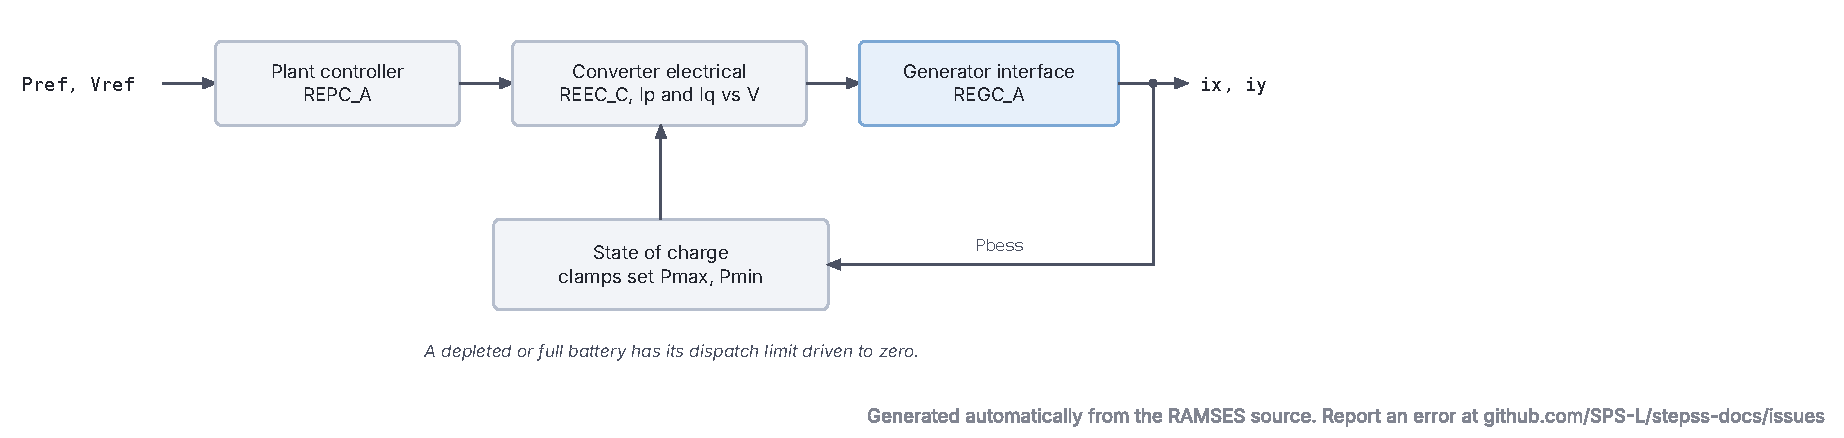
\includegraphics[width=0.98\linewidth]{figures/inj-bess-light}
\caption{Battery energy storage block diagram.}
\end{figure}

\subsubsection{Parameters (key parameters)}\label{model-inj:parameters-key-parameters}

\begin{small}\begin{longtable}[]{@{}
  >{\raggedright\arraybackslash}p{(\linewidth - 10\tabcolsep) * \real{0.1349}}
  >{\raggedright\arraybackslash}p{(\linewidth - 10\tabcolsep) * \real{0.1752}}
  >{\raggedright\arraybackslash}p{(\linewidth - 10\tabcolsep) * \real{0.1660}}
  >{\raggedright\arraybackslash}p{(\linewidth - 10\tabcolsep) * \real{0.3870}}
  >{\raggedright\arraybackslash}p{(\linewidth - 10\tabcolsep) * \real{0.1368}}
@{}}
\toprule\noalign{}
\begin{minipage}[b]{\linewidth}\raggedright
\#
\end{minipage} & \begin{minipage}[b]{\linewidth}\raggedright
Name
\end{minipage} & \begin{minipage}[b]{\linewidth}\raggedright
Sub-model
\end{minipage} & \begin{minipage}[b]{\linewidth}\raggedright
Description
\end{minipage} & \begin{minipage}[b]{\linewidth}\raggedright
Unit
\end{minipage} \\
\midrule\noalign{}
\endhead
\bottomrule\noalign{}
\endlastfoot
1 & \texttt{SNOM} & & Nominal power & MW \\
2--32 & & REPC\_A & Plant controller (same as WT3/WT4) & various \\
33--76 & & REEC\_C & Electrical controller with piecewise \(I_q(V)\), \(I_p(V)\) & various \\
68 & \texttt{CapBat} & BESS & Battery energy capacity & MWh \\
69 & \texttt{SOCini} & BESS & Initial state of charge & pu \\
70 & \texttt{SOCmax} & BESS & Maximum SOC limit & pu \\
71 & \texttt{SOCmin} & BESS & Minimum SOC limit & pu \\
72--73 & \texttt{dPmax}, \texttt{dPmin} & BESS & Active power ramp rate limits & pu/s \\
74--75 & \texttt{pmax}, \texttt{pmin} & REEC\_C & Active current limits (pu on SNOM) & pu \\
76 & \texttt{Tpord} & REEC\_C & Active power order time constant & s \\
\end{longtable}\end{small}

Full parameter listing has approximately 125 parameters; refer to a working example data file for the complete ordering.

\subsubsection{State Variables}\label{model-inj:state-variables-11}

The BESS model uses over 40 internal states reflecting the three sub-models. Key states include:

\begin{small}\begin{longtable}[]{@{}ll@{}}
\toprule\noalign{}
Variable & Description \\
\midrule\noalign{}
\endhead
\bottomrule\noalign{}
\endlastfoot
\texttt{SOC} & State of charge \\
\texttt{Pref} & Active power reference \\
\texttt{Qext} & Reactive power reference from REPC\_A \\
\texttt{Ip}, \texttt{Iq} & Active/reactive current outputs \\
\texttt{PLLPhaseAngle} & PLL phase angle \\
\texttt{Pgen}, \texttt{Qgen} & Generated powers \\
\end{longtable}\end{small}

\subsubsection{Usage Example}\label{model-inj:usage-example-14}

\begin{Verbatim}
INJEC  BESS  BESS1  BUS_ST  1.  1.  0.  0.
    100.0  0.0  0.02  0  0.0  0.05  0  0.0  0.3  -0.3  2.0  0.4
    0.3  -0.3  0.0  0.15  0.9  0.05  0.0  -0.06  0.06  -0.05  0.05
    0.05  -0.05  2.0  1.0  1.0  -1.0  0.02  0  0
    0.1  0.1  0.02  1.0  0.0  -0.2  0.2  0.2  -0.2  0.6  0.4  0.6  -0.6  1.1  0.9
    1.0  0.5  0.01  0.01  0.05  0.9  0.2  0.9  0.1  0.9  -0.1  0.5  -0.5  0.5  -0.5  1.0  -1.0  0.5  -0.5
    50.0  0.7  0.9  0.1  5.0  -5.0  1.0  -1.0  0.05  1.1  0.0  2  0.01  ;
\end{Verbatim}

\begin{center}\rule{0.5\linewidth}{0.5pt}\end{center}

\section{Reactive Compensation}\label{model-inj:reactive-compensation}

\subsection{\texorpdfstring{SVC\_GENERIC1 (\texttt{inj\_svc\_generic1}): Generic Static Var Compensator}{SVC\_GENERIC1 (inj\_svc\_generic1): Generic Static Var Compensator}}\label{model-inj:svc_generic1-inj_svc_generic1-generic-static-var-compensator}

The data-file model name is \texttt{SVC\_GENERIC1}. It takes no prefix.

\subsubsection{Description}\label{model-inj:description-15}

A dynamic SVC injecting a purely reactive current at its bus. A PI voltage
regulator with droop drives a susceptance \(B_{svc}\) between \texttt{Bmin} and \texttt{Bmax},
and two lead-lag stabiliser channels can add a supplementary signal to the
voltage reference. This is the dynamic counterpart of the static
\hyperref[ch-pf]{SVC record} used by the
power flow: the static record fixes the operating point, this model governs how
the device behaves during the simulation.

The voltage reference is initialised from the power flow solution, so that the
model starts in equilibrium:

\[V_{ref} = V_0 + B_p \cdot B_{svc,0}\]

where \(B_p\) is the droop and \(B_{svc,0}\) the initial susceptance implied by the
reactive current at the bus.

\begin{figure}[htbp]
\centering
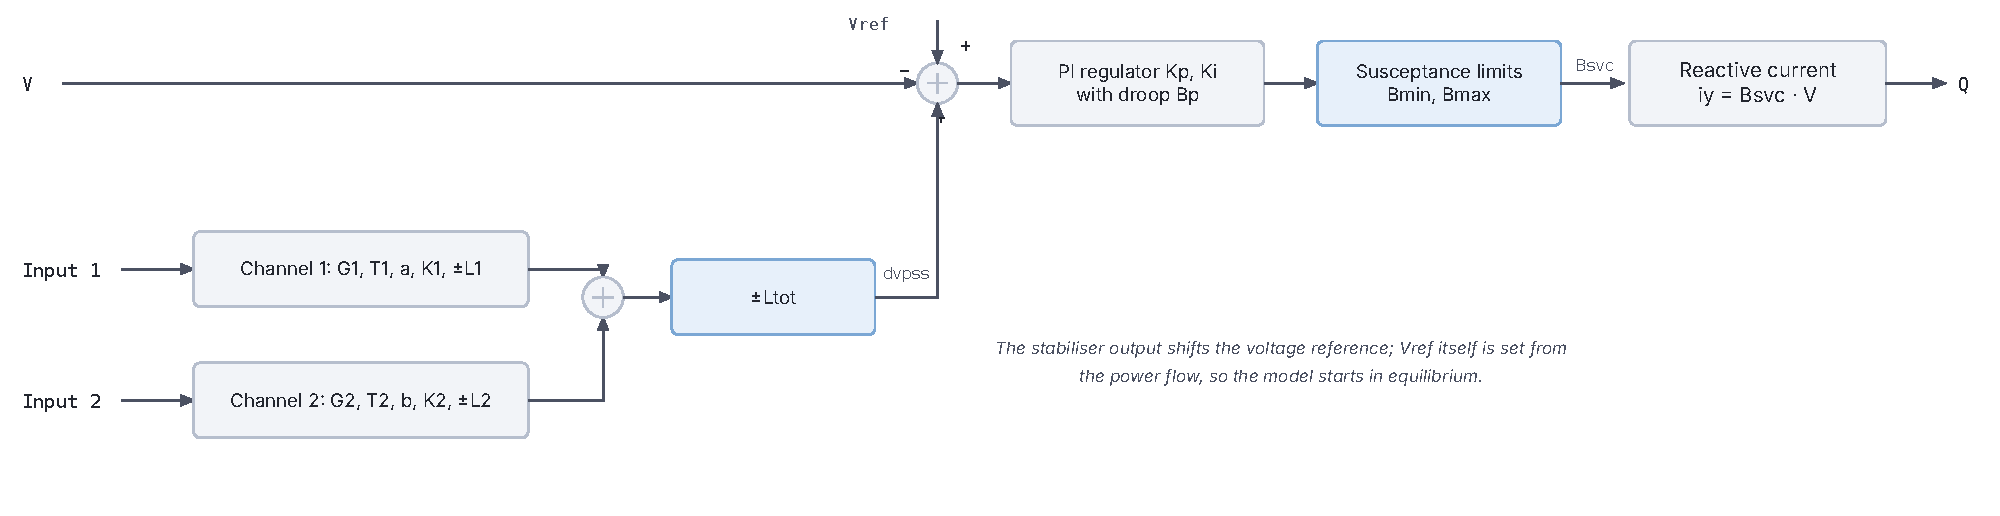
\includegraphics[width=0.98\linewidth]{figures/inj-svc-generic1-light}
\caption{Generic static var compensator block diagram.}
\end{figure}

\subsubsection{Parameters}\label{model-inj:parameters-11}

The record carries 17 data parameters, in order:

\begin{small}\begin{longtable}[]{@{}
  >{\raggedright\arraybackslash}p{(\linewidth - 6\tabcolsep) * \real{0.1337}}
  >{\raggedright\arraybackslash}p{(\linewidth - 6\tabcolsep) * \real{0.1739}}
  >{\raggedright\arraybackslash}p{(\linewidth - 6\tabcolsep) * \real{0.6925}}
@{}}
\toprule\noalign{}
\begin{minipage}[b]{\linewidth}\raggedright
\#
\end{minipage} & \begin{minipage}[b]{\linewidth}\raggedright
Name
\end{minipage} & \begin{minipage}[b]{\linewidth}\raggedright
Description
\end{minipage} \\
\midrule\noalign{}
\endhead
\bottomrule\noalign{}
\endlastfoot
1 & \texttt{G1} & Gain of the first stabiliser channel \\
2 & \texttt{T1} & Time constant of the first stabiliser channel (s) \\
3 & \texttt{a} & Lead-lag coefficient of the first channel \\
4 & \texttt{K1} & Output gain of the first channel \\
5 & \texttt{L1} & Output limit of the first channel (pu) \\
6 & \texttt{G2} & Gain of the second stabiliser channel \\
7 & \texttt{T2} & Time constant of the second stabiliser channel (s) \\
8 & \texttt{b} & Lead-lag coefficient of the second channel \\
9 & \texttt{K2} & Output gain of the second channel \\
10 & \texttt{L2} & Output limit of the second channel (pu) \\
11 & \texttt{Ltot} & Limit on the summed stabiliser output (pu) \\
12 & \texttt{Kp} & Proportional gain of the voltage regulator \\
13 & \texttt{Ki} & Integral gain of the voltage regulator \\
14 & \texttt{Bp} & Droop, in pu on the SVC base \\
15 & \texttt{Bmax} & Maximum susceptance (Mvar at 1 pu voltage) \\
16 & \texttt{Bmin} & Minimum susceptance (Mvar at 1 pu voltage) \\
17 & \texttt{Bnom} & Susceptance base used for the per-unit conversion (Mvar) \\
\end{longtable}\end{small}

One additional parameter is computed at initialisation:

\begin{small}\begin{longtable}[]{@{}lll@{}}
\toprule\noalign{}
\# & Name & Description \\
\midrule\noalign{}
\endhead
\bottomrule\noalign{}
\endlastfoot
18 & \texttt{Vref} & Voltage reference, set from the power flow solution \\
\end{longtable}\end{small}

\subsubsection{Observables}\label{model-inj:observables}

\texttt{Q}, \texttt{dvpss}, \texttt{Bsvc}, \texttt{Vref}, \texttt{Vb}

\begin{center}\rule{0.5\linewidth}{0.5pt}\end{center}

\section{Measurement}\label{model-inj:measurement}

\subsection{\texorpdfstring{PMU (\texttt{inj\_PMU}): Phasor Measurement Unit}{PMU (inj\_PMU): Phasor Measurement Unit}}\label{model-inj:pmu-inj_pmu-phasor-measurement-unit}

The data-file model name is \texttt{PMU} (or \texttt{inj\_PMU}).

\subsubsection{Description}\label{model-inj:description-16}

A measurement-only injector: it injects \textbf{zero current} at its bus and exists
purely to expose bus quantities as observables. It reports a filtered local
frequency estimate computed the same way as the \texttt{f\_inj} block, together with the
bus voltage magnitude and angle and the speed and angle of the moving DQ
reference frame. Attach one to any bus whose frequency you want to record
without perturbing the solution.

The frequency estimate is a first-order filter on the bus voltage phasor. The
measurement time constant is clamped to a floor of 0.05 s, so values below that
have no effect.

\subsubsection{Parameters}\label{model-inj:parameters-12}

\begin{small}\begin{longtable}[]{@{}
  >{\raggedright\arraybackslash}p{(\linewidth - 8\tabcolsep) * \real{0.0870}}
  >{\raggedright\arraybackslash}p{(\linewidth - 8\tabcolsep) * \real{0.1508}}
  >{\raggedright\arraybackslash}p{(\linewidth - 8\tabcolsep) * \real{0.6246}}
  >{\raggedright\arraybackslash}p{(\linewidth - 8\tabcolsep) * \real{0.1376}}
@{}}
\toprule\noalign{}
\begin{minipage}[b]{\linewidth}\raggedright
\#
\end{minipage} & \begin{minipage}[b]{\linewidth}\raggedright
Name
\end{minipage} & \begin{minipage}[b]{\linewidth}\raggedright
Description
\end{minipage} & \begin{minipage}[b]{\linewidth}\raggedright
Unit
\end{minipage} \\
\midrule\noalign{}
\endhead
\bottomrule\noalign{}
\endlastfoot
1 & \texttt{Tf} & Frequency measurement time constant, recommended 0.05 to 0.10; values below 0.05 are clamped & s \\
\end{longtable}\end{small}

Three additional parameters are set at initialisation: \texttt{wnom} (nominal angular
frequency), \texttt{vm0} and \texttt{va0} (the initial bus voltage magnitude and angle).

\subsubsection{Observables}\label{model-inj:observables-1}

\begin{small}\begin{longtable}[]{@{}
  >{\raggedright\arraybackslash}p{(\linewidth - 6\tabcolsep) * \real{0.1648}}
  >{\raggedright\arraybackslash}p{(\linewidth - 6\tabcolsep) * \real{0.6281}}
  >{\raggedright\arraybackslash}p{(\linewidth - 6\tabcolsep) * \real{0.2071}}
@{}}
\toprule\noalign{}
\begin{minipage}[b]{\linewidth}\raggedright
Name
\end{minipage} & \begin{minipage}[b]{\linewidth}\raggedright
Description
\end{minipage} & \begin{minipage}[b]{\linewidth}\raggedright
Unit
\end{minipage} \\
\midrule\noalign{}
\endhead
\bottomrule\noalign{}
\endlastfoot
\texttt{f} & Estimated bus frequency & pu of \(f_{nom}\) \\
\texttt{vm} & Bus voltage magnitude & pu \\
\texttt{va} & Bus voltage phase angle in the moving DQ frame, wrapping at \(\pm\pi\) & rad \\
\texttt{thref} & Accumulated angle of the DQ reference frame with respect to the nominally rotating frame, zero at \(t = 0\) & rad \\
\texttt{dwref} & Speed deviation of the DQ reference frame from nominal & rad/s \\
\end{longtable}\end{small}

\begin{docsnote}{Caution}

\texttt{dwref} and \texttt{thref} are only meaningful under \texttt{\$OMEGA\_REF\ COI}. With
\texttt{\$OMEGA\_REF\ SYN} the reference frame rotates at nominal speed by construction,
so both stay at zero.

\end{docsnote}

\subsubsection{Usage Example}\label{model-inj:usage-example-15}

\begin{Verbatim}
INJEC  PMU  PMU_1041  1041  0.  0.  0.  0.  0.05 ;
\end{Verbatim}

All four participation and power fields are zero: the model neither consumes nor
produces power.
